%% History:
% Pavel Tvrdik (26.12.2004)
%  + initial version for PhD Report
%
% Daniel Sykora (27.01.2005)
%
% Michal Valenta (3.12.2008)
% rada zmen ve formatovani (diky M. Duškovi, J. Holubovi a~J. Žďárkovi)
% sjednoceni zdrojoveho kodu pro anglickou, ceskou, bakalarskou a~diplomovou praci

% One-page layout: (proof-)reading on displa
%%%% \documentclass[11pt,oneside,a4paper]{book}
% Two-page layout: final printing
\documentclass[11pt,twoside,a4paper]{book}   

%=-=-=-=-=-=-=-=-=-=-=-=--=%
% The user of this template may find useful to have an alternative to these 
% officially suggested packages:
\usepackage[czech, english]{babel}
%\usepackage[T1]{fontenc} % pouzije EC fonty 
% pripadne pisete-li cesky, pak lze zkusit take:
\usepackage[T1]{fontenc}
\usepackage{lmodern}
%\usepackage[cp1250]{inputenc}
\usepackage[utf8x]{inputenc}

\usepackage{listings}
% Pozicovani
\usepackage{float}
\restylefloat{table}

%=-=-=-=-=-=-=-=-=-=-=-=--=%
% In case of problems with PDF fonts, one may try to uncomment this line:
%\usepackage{lmodern}
%=-=-=-=-=-=-=-=-=-=-=-=--=%
%=-=-=-=-=-=-=-=-=-=-=-=--=%
% Depending on your particular TeX distribution and version of conversion tools 
% (dvips/dvipdf/ps2pdf), some (advanced | desperate) users may prefer to use 
% different settings.
% Please uncomment the following style and use your CSLaTeX (cslatex/pdfcslatex) 
% to process your work. Note however, this file is in UTF-8 and a~conversion to 
% your native encoding may be required. Some settings below depend on babel 
% macros and should also be modified. See \selectlanguage \iflanguage.
%\usepackage{czech}  %%%%%\usepackage[T1]{czech} %%%%[IL2] [T1] [OT1]
%=-=-=-=-=-=-=-=-=-=-=-=--=%

%%%%%%%%%%%%%%%%%%%%%%%%%%%%%%%%%%%%%%%
% Styles required in your work follow %
%%%%%%%%%%%%%%%%%%%%%%%%%%%%%%%%%%%%%%%
\usepackage{graphicx}
%\usepackage{indentfirst} %1. odstavec jako v~cestine.

\usepackage{k336_thesis_macros} % specialni makra pro formatovani DP a~BP
 % muzete si vytvorit i~sva vlastni v~souboru k336_thesis_macros.sty
 % najdete  radu jednoduchych definic, ktere zde ani nejsou pouzity
 % napriklad: 
 % \newcommand{\bfig}{\begin{figure}\begin{center}}
 % \newcommand{\efig}{\end{center}\end{figure}}
 % umoznuje pouzit prikaz \bfig namisto \begin{figure}\begin{center} atd.

\newcommand{\declarationn}[1]{
\cleardoublepage
\vspace*{\fill}
\noindent
{\huge \textbf{%
{Prohlášení}
}}
\vspace{3ex}\par
\noindent
Prohlašuji, že jsem práci vypracoval samostatně a použil jsem pouze podklady uvedené v~přiloženém seznamu.\\
Nemám závažný důvod proti užití tohoto školního díla ve smyslu \S 60 Zákona č.~121/2000 Sb., o právu autorském, o právech souvisejících s právem autorským a o změně některých zákonů (autorský zákon).%
\\[15mm]
#1 \hfill \hbox to 70mm{\tiny\dotfill}
}

\newcommand{\acknowledgementss}{
\cleardoublepage
\vspace*{\fill}
\noindent
{\huge \textbf{%
{Poděkování}
}}
\vspace{3ex}\par
}


\usepackage{indentfirst}

%%%%%%%%%%%%%%%%%%%%%%%%%%%%%%%%%%%%%
% Zvolte jednu z moznosti 
% Choose one of the following options
%%%%%%%%%%%%%%%%%%%%%%%%%%%%%%%%%%%%%
\newcommand\TypeOfWork{Diplomová Práce}  \typeout{Diplomova prace}


%%%%%%%%%%%%%%%%%%%%%%%%%%%%%%%%%%%%%
% Zvolte jednu z moznosti 
% Choose one of the following options
%%%%%%%%%%%%%%%%%%%%%%%%%%%%%%%%%%%%%
% nabidky jsou z: http://www.fel.cvut.cz/cz/education/bk/prehled.html

\newcommand\StudProgram{Otevřená informatika, Magisterský}

%%%%%%%%%%%%%%%%%%%%%%%%%%%%%%%%%%%%%
% Zvolte jednu z moznosti 
% Choose one of the following options
%%%%%%%%%%%%%%%%%%%%%%%%%%%%%%%%%%%%%
% nabidky jsou z: http://www.fel.cvut.cz/cz/education/bk/prehled.html

\newcommand\StudBranch{Počítačová grafika a interakce} %..

%%%%%%%%%%%%%%%%%%%%%%%%%%%%%%%%%%%%%%%%%%%%
% Vyplnte nazev prace, autora a~vedouciho
% Set up Work Title, Author and Supervisor
%%%%%%%%%%%%%%%%%%%%%%%%%%%%%%%%%%%%%%%%%%%%

\newcommand\WorkTitle{Jazyk pro definici uživatelského rohzaní}%..
\newcommand\FirstandFamilyName{Bc. Michal Hotovec}
\newcommand\Supervisor{Ing. Tomáš Barák}


% Pouzijete-li pdflatex, tak je prijemne, kdyz bude mit vase prace
% funkcni odkazy i~v pdf formatu
\usepackage[hyphens]{url}
\usepackage[
pdftitle={\WorkTitle},
pdfauthor={\FirstandFamilyName},
bookmarks=true,
colorlinks=true,
breaklinks=true,
urlcolor=blue,
citecolor=blue,
linkcolor=blue,
unicode=true,
]
{hyperref}


% Extension posted by Petr Dlouhy in order for better sources reference (\cite{} command) especially in Czech.
% April 2010
% See comment over \thebibliography command for details.

\usepackage[square, numbers]{natbib}             % sazba pouzite literatury
%\DeclareUrlCommand\url{\def\UrlLeft{<}\def\UrlRight{>}\urlstyle{tt}}  %rm/sf/tt
%\renewcommand{\emph}[1]{\textsl{#1}}    % melo by byt kurziva nebo sklonene,
%\let\oldUrl\url
%\renewcommand\url[1]{<\texttt{\oldUrl{#1}}>}


\usepackage{fancyhdr}

\begin{document}


\selectlanguage{czech} 


 \typeout{************************************************}
	 \typeout{Zvoleny jazyk: cestina}
	 \typeout{Typ prace: \TypeOfWork}
	 \typeout{Studijni program: \StudProgram}
	 \typeout{Obor: \StudBranch}
	 \typeout{Jmeno: \FirstandFamilyName}
	 \typeout{Nazev prace: \WorkTitle}
	 \typeout{Vedouci prace: \Supervisor}
	 \typeout{***************************************************}
	 \newcommand\Department{Katedra počítačové grafiky a interakce}
	 \newcommand\Faculty{Fakulta elektrotechnická}
	 \newcommand\University{České vysoké učení technické v~Praze}
	 \newcommand\labelSupervisor{Vedoucí práce}
	 \newcommand\labelStudProgram{Studijní program}
	 \newcommand\labelStudBranch{Obor}



\pagenumbering{roman} \cleardoublepage \thispagestyle{empty}

\chapter*{Jazyk pro definici uživatelského rozhraní}

\begin{itemize}
\item Prostudujte nástroje pro tvorbu moderních grafických uživatelských rozhraní. Zaměřte se na jazyk \textit{QML}.
\item Navrhněte jazyk syntakticky co nejvíce podobný \textit{QML} přímo integrovatelný do \textit{C/C++} aplikace.
\item Navržený jazyk popište gramatikou a implementujte jeho překladač do pomocného \textit{C/C++} kódu.
\item Implementujte podpůrnou knihovnu pro běh grafických aplikací napsaných navrženým jazykem.
%\item Výsledky předveďte na \textit{C/C++} aplikaci obsahující uživatelské rozhraní naprogramované navrženým jazykem.
\item Diskutujte výhody a nevýhody navrženého řešení, řešení porovnejte s \textit{QML}.
\end{itemize}
\newpage
\thispagestyle{plain}

\coverpagestarts

\acknowledgementss
\noindent
%T�mto bych r�d pod�koval vedoucimu

\declarationn{V Pečkách dne 10.\,5.\,2015} 
%..

%\begin{frontmatter}

%\title{Diplomová práce\\ Jazyk pro definici uživatelského rozhraní}

%\author{Michal Hotovec\footnote{A4M39SVP -- Michal Hotovec, zimní semestr 2014/15}\\
%Katedra pořítačové grafiky a interakce,\\ Fakulta elektrotechnická, ČVUT Praha
%}


%%%\date{}


\abstractpage
%..
English abstract

% Prace v~cestine musi krome abstraktu v~anglictine obsahovat i
% abstrakt v~cestine.
\vglue60mm

\noindent{\Huge \textbf{Abstrakt}}
\vskip 2.75\baselineskip

\noindent
Český abstrakt


\noindent


%\end{frontmatter}


%%%%%%%%%%%%%%%%%%%%%%%%%%%%%%%%  Obsah / Table of Contents 
\setcounter{secnumdepth}{2}
\setcounter{tocdepth}{1}
\tableofcontents


\listoffigures

% list kodu ..
%\listoftables

%\maketitle

%% \input{./section1.tex}
%% \input{./section2.tex}
%% \input{./section3.tex}
%% \input{./section4.tex}
%% \input{./section5.tex}

\mainbodystarts
% horizontalní mezera mezi dvema odstavci
%\parskip=5pt
%11.12.2008 parskip + tolerance
\normalfont
\parskip=0.2\baselineskip plus 0.2\baselineskip minus 0.1\baselineskip



%%%% -------------------------------------------------------- 

\chapter{\label{CH:Intro}Úvod}
%\section{\label{SEC:Intro}Introduction}
Cílem této práce je vytvořit jazyk pro tvorbu grafického uživatelského rozhraní (\textit{GUI}), který by poskytoval funkčnost podobnou jazyku \textit{QML}. Ale oproti jazyku \textit{QML}, který je interpretovaný, půjde vytvořený jazyk přeložit do zkompilovatelného kódu \textit{C/C++}. Součástí práce je také bylo vytvořit překladač pro daný jazyk, který ověří validitu vstupu a přeloží jej do kódu \textit{C/C++}, který půjde integrovat do \textit{C/C++} aplikace a spustit. Tato aplikace by následně měla zobrazit \textit{GUI} definované v navrženém jazyce.\\
Pro účely správy \textit{GUI} v rámci uživatelské aplikace, je nutné implementovat podpůrnou knihovnu, kterou bude uživatelská aplikace používat. Aby tato knihovna mohla být používána na co nejvíce platformách, podporuje vyměnitelné externí rozhraní pro vstup a výstup, který je následně implementován v rámci uživatelské aplikace.\\
Na závěr práce je vytvořeno jednoduché \textit{GUI} v jazyce \textit{QML} i nově navrženém jazyce, na čemž je demonstrována podobnost i rozdíly mezi jednotlivými řešeními.





\chapter{\label{CH:Rash}Rešerše}

\section{\label{SEC:history}Historie \textit{GUI}}
\subsection{Počátky \textit{GUI}}
Za počátek vzniku disciplíny vývoje uživatelského rozhraní pro počítače je považováno publikování článku \textit{Augmenting Human Intellect} od D. C. Engelbarta v roce 1962 (\cite{bib:AHI}). Kde autor argumentoval, že schopnost lidského intelektu zkoumat a řešit komplexní problémy a situace může být rozšířena pomocí vhodných nástrojů, v tomto případě počítačů. V zápětí bylo založen výzkumné centrum Augmentation Human Intellect (\textit{AHI}) Research Center (také známé pod zkratkou \textit{ARC}) ve Stanfordském výzkumném institutu, které fungovalo až do roku 1989, kdy byla jeho činnost ukončena z finančních důvodů. V rámci centra \textit{AHI} započal vývoj experimentálních technologií pro rozšíření schopností lidského intelektu.\\
6. prosince 1968 byly veřejně předvedeny vyvinuté technologie ve formě \textit{NLS} (\textit{oN-Line System}) na konferenci \textit{Fall Joint Computer Conference} v San Franciscu. Na tomto systému byl demonstrován nový přístup k interakci uživatele s počítačem. Jednalo se o distribuovaný systém několika počítačů. Pro vstup uživatele bylo používáno několik zařízení, konkrétně klávesnice, několik posuvníků a úplně první počítačové myši. Systém používal komerčně dostupný displej, který umožňoval vykreslování znaků a vektorové zobrazení grafiky v podobě čar. Ukazatel myši byl na obrazovce zobrazen pomocí svislé šipky. Během ukázky bylo demonstrováno sdílení grafického výstupu na více obrazovek . Dále zde byla demonstrována úprava dokumentů, možnosti jejich zobrazování a úpravy jejich hierarchie. Z technologií a přístupů prezentovaných v rámci ukázky tohoto systému vyšly v budoucnosti, některé společnosti při návrhu svých uživatelských rozhraní.\cite{bib:aug}\\
\subsection{První \textit{GUI}}
V roce 1970 byl společností \textit{Xerox} založen výzkumný institut \textit{PARC} (\textit{Palo Alto Research Center}). Během prvních let fungování bylo vyvinuto několik dodnes využívaných technologií, mezi něž patří i technologie laserového tisku vyvinutá v roce 1971. 
\begin{figure*}[!ht]
\begin{center}
  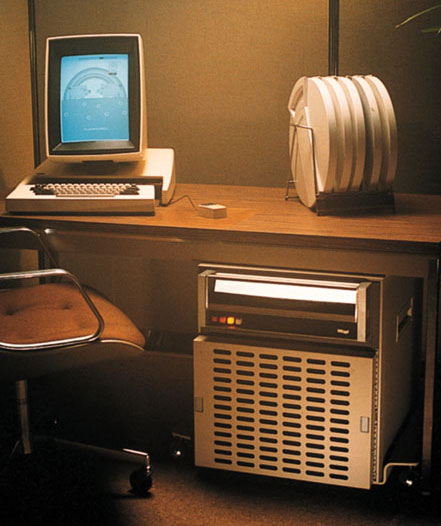
\includegraphics[width=0.7\textwidth]{XeroxAlto}
\caption{{\label{fig:alto}}Počítač Xerox Alto.}
\end{center}
\end{figure*}
%obr. alto http://history-computer.com/ModernComputer/Personal/Alto.html
V tehdejší době neexistovaly počítače, které by umožnily manipulaci s podobou tištěných dokumentů, pomocí jiného než textové rozhraní. Proto byl v PARC zahájen vývoj počítače, který byl v roce 1973 světu představen jako počítač \textit{Alto Personal Workstation}. Tento počítač byl během let postupně vylepšován a postupně se stal prvním počítačem, který používal bitmapový displej a umožnil grafickou úpravu dokumentů. V roce 1972 byl v institutu \textit{PARC} vyvinut první objektově orientovaný jazyk zvaný \textit{SmallTalk}, který umožňoval jednotlivé součásti programu rozdělit do samostatných objektů, které mohli být následně používány i v jiných programech. V roce 1975 bylo vyvinuto první \textit{GUI}, které se svou funkčností velice podobalo dnešnímu. Zahrnovalo mimo jiné ikony, překrývající se okna, vyskakovací nabídky a mohla být ovládáno pomocí myši. \cite{bib:PARC}
\begin{figure*}[!ht]
\begin{center}
  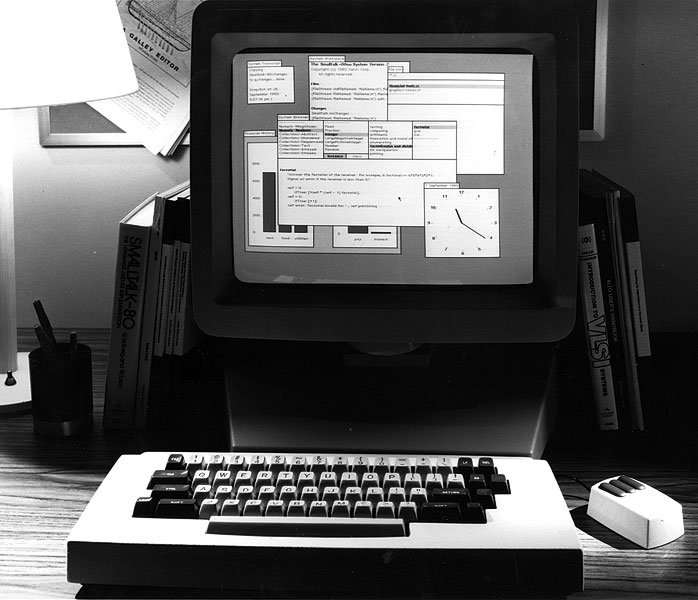
\includegraphics[width=0.7\textwidth]{altost2}
\caption{{\label{fig:altoGUI}}Počítač Xerox Alto, nekterém běží jedno z prvních GUI.}
\end{center}
\end{figure*}
% obr. gui http://toastytech.com/guis/alto3.html
Počítač \textit{Alto} však nebyl nikdy komerčně k dispozici a až v roce 1981 byla dána veřejně k prodeji jeho variace pod názvem \textit{Xerox Star 8010 Document Processor}.

\subsection{Rozvoj v osmdesátých letech}
V osmdesátých letech dvacátého století se začaly na trhu objevovat první počítače poskytující \textit{GUI}.\cite{bib:history}
\subsubsection{Apple}
Za jednoho z dalších průkopníků je považována společnost \textit{Apple} založená v roce 1976. Která za svůj počáteční úspěch vděčila populárnímu počítači \textit{Apple ][}, který umožňoval zobrazení textu i grafiky, avšak poskytoval pouze textové vstupní rozhraní. Společnost byla ovlivněna vlivem institutu \textit{PARC} a započala v roce 1979 vývoj počítače \textit{Lisa}, který měl být jejím prvním počítačem poskytující ovládání pomocí \textit{GUI}. Vývoj tohoto počítače byl dokončen v roce 1983. Díky vysoké ceně však nebyl počítač příliš komerčně úspěšný a v ruce 1984 byla trhu představena jeho levnější verze - počítač \textit{Macintosh}, který ačkoli měl nižší výkon než \textit{Lisa}, zachoval většinu schopností jejího \textit{GUI}.
\begin{figure*}[!ht]
\begin{center}
  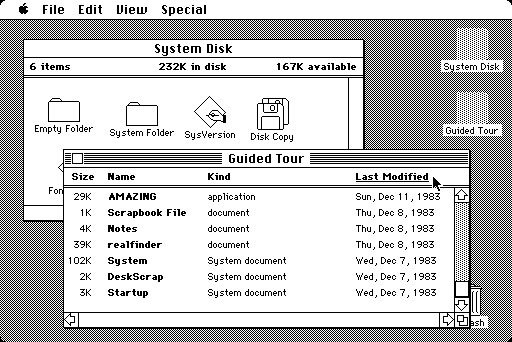
\includegraphics[width=0.7\textwidth]{mac}
\caption{{\label{fig:macGUI}} Grafické rozhraní počítače Macintosh.}
\end{center}
\end{figure*}
%http://history-computer.com/ModernComputer/Personal/Macintosh.html
\subsubsection{Microsoft Windows}
V roce 1983 Microsoft ohlásil vývoj systému \textit{Windows 1.0}, který byl dokončen v roce 1985. Na rozdíl od moderních rozhranní, tento systém používal okna, která byla ve svých vyhrazených prostorech na obrazovce a nemohla překrývat. V roce 1987 byla vydána verze \textit{Windows 2.0}, která zavedla tradiční systém překrývajících se oken, která se dala přesunovat pomocí myši.
\begin{figure*}[!ht]
\begin{center}
  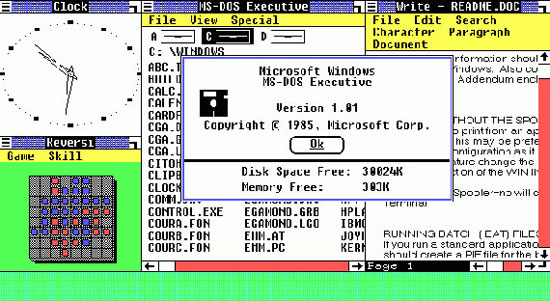
\includegraphics[width=0.4\textwidth]{win1}
\caption{{\label{fig:win1GUI}} Grafické rozhraní systému Windows 1.0.}
\end{center}
\end{figure*}
%http://history-computer.com/ModernComputer/Software/Windows.html
\begin{figure*}[!ht]
\begin{center}
  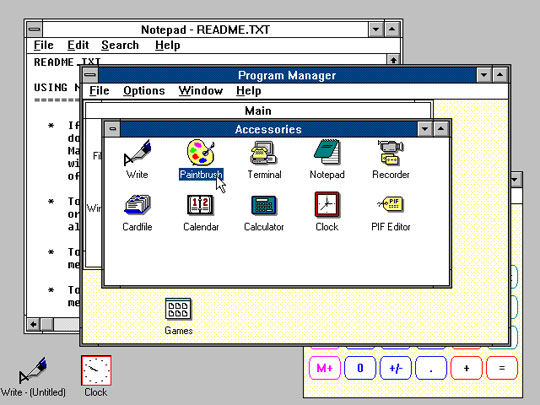
\includegraphics[width=0.4\textwidth]{win2}
\caption{{\label{fig:win2GUI}} Grafické rozhraní systému Windows 2.0.}
\end{center}
\end{figure*}
% http://history-computer.com/ModernComputer/Software/Windows.html

\subsubsection{Amiga Workbench}
V roce 1985 společnost \textit{Commodore} představila počítač \textit{Amiga}, který poskytoval své \textit{GUI} \textit{Amiga Workbench}. Toto rozhranní umožňovalo ručně přehazovat pořadí oken na obrazovce (odpředu dozadu) a umožňovalo manipulovat pomocí myši s jednotlivými okny tradičním způsobem. Díky manuálnímu způsobu pořadí vykreslování oken, bylo umožněno pracovat s oknem, aniž by se přesunulo dopředu.
\begin{figure*}[!ht]
\begin{center}
  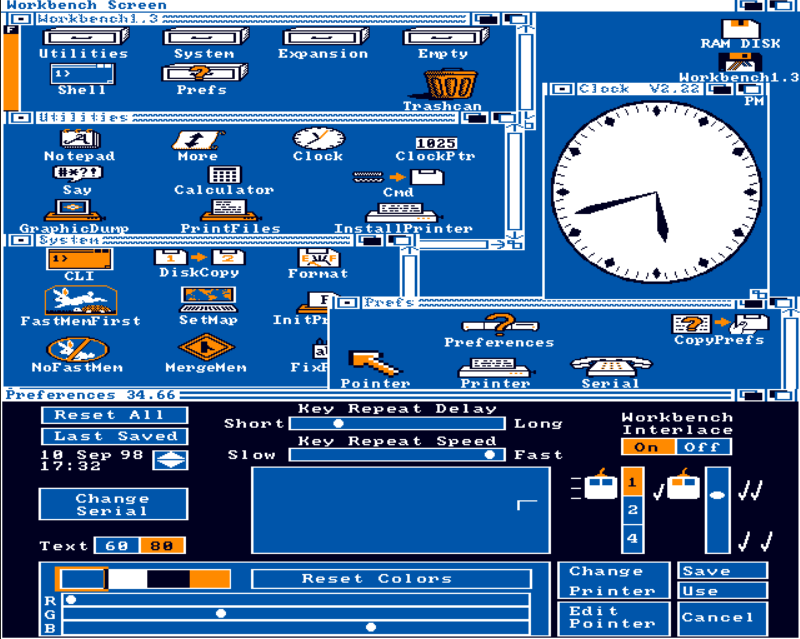
\includegraphics[width=0.7\textwidth]{amiga}
\caption{{\label{fig:amigaGUI}} Grafické rozhraní počítače Amiga Workbench.}
\end{center}
\end{figure*}
%http://www.gregdonner.org/workbench/wb_13.html

\subsubsection{Acorn}
V roce 1987 společnost \textit{Acorn Computers} vyvinula své \textit{GUI} zvané \textit{Arthur}, které jako první umožnilo zobrazení fontů v šestnácti barvách s použitím anti-aliasingu.
\begin{figure*}[!ht]
\begin{center}
  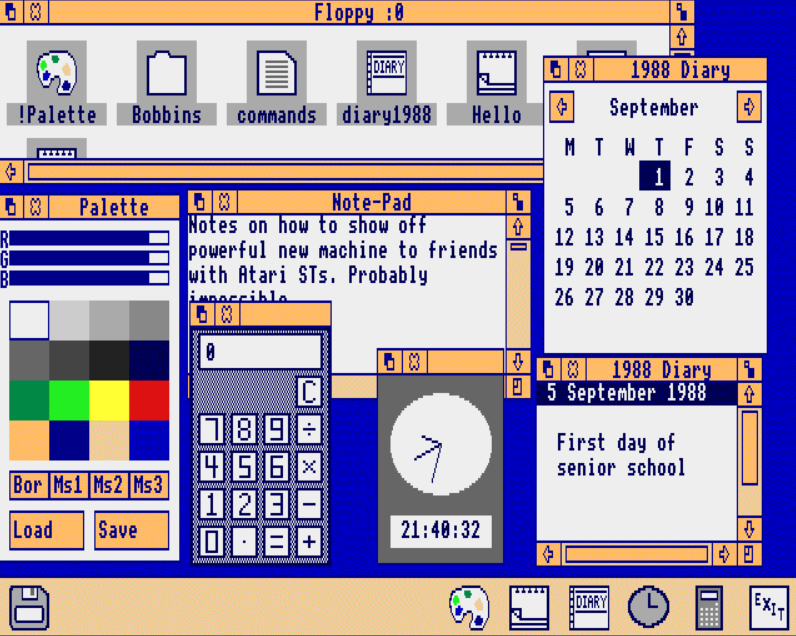
\includegraphics[width=0.7\textwidth]{arthur}
\caption{{\label{fig:arthurGUI}} Grafické rozhraní Arthur společnosti Acorn Computers.}
\end{center}
\end{figure*}
% http://toastytech.com/guis/guitimeline2.html
\section{\label{SEC:modelGUI}Tvorba \textit{GUI} pomocí deklarativních modelů}
Podobně jako u programování běžných aplikací existuje deklarativní a imperativní přístup k tvorbě \textit{GUI} aplikací. Imperativní přístup spočívá v tom, že programátor v rámci aplikačního kódu přímo naprogramuje struktury uživatelského rozhraní, spolu s jejich funkčností a vzhledem.\\
Jelikož předmětem této práce je vyjít z existujícího deklarativním jazyka pro tvorbu \textit{GUI}, bude se zabývat především tvorbou \textit{GUI} pomocí deklarativních modelů. Základem tohoto přístupu je, že vývojář popíše vzhled a strukturu \textit{GUI} pomocí nějakého modelu. Model obsahuje informace nutné pro vytvoření samotného uživatelského rozhraní. Tento model je přístupný aplikaci, která podle něj vytvoří deklarované uživatelské rozraní.
%// obrázek
Existuje několik běžně užívaných modelů pro deklarativní tvorbu \textit{GUI}.
\begin{itemize}
\item Datové modely
Datové modely byly prvními používanými modely v rámci modelově založeného vývoje \textit{GUI}. Jsou přímo odvozeny z datových struktur aplikace, proto jsou zejména užitečné při generování \textit{GUI} výběrem součástí podle toho, z jakého typu byly odvozeny. Některé systémy dokážou z datového modelu pomocí algoritmů přímo vygenerovat úplné uživatelské rozhraní. \cite{bib:model2}
\item Doménové modely
Doménový model representuje objekty v doméně a jejich vzájemné vztahy. Patří mezi ně některé objektově orientované datové modely. Tyto modely vedly k plně deklarativním doménovým modelům, které dokáží efektivně popsat vztahy mezi objekty jednotlivých domén a umožňují generování \textit{GUI} s dynamickým chováním v rámci statického rozvržení.
\item Aplikační modely
Specifikují služby, které aplikace poskytuje. Zpravidla se jedná o objektově orientované modely. Kde objekty uchovávají stav jednotlivých součástí v rámci \textit{GUI} a také operací, které ovlivňují stav těchto součástí. Cílem těchto modelů je usnadnit deklaraci chování \textit{GUI}.
\item User-task model
Tento model je součástí user-centered design (designu cíleného na uživatele). Popisuje úkony, které koncový uživatel může provádět a jaké interakční možnosti musí být navrženy. Model zahrnuje prvky, jako jsou cíle, úkony, a doménové objekty. Cíle definují požadované stavy. Sekvence úkonů definuje proceduru k dosažení určitého cíle. Doménové objekty reprezentují jednotlivé elementy, které musí být zobrazeny v rámci provedení jednotlivých úkonů.
\item Dialogový model
Dialogový model popisuje komunikace člověk-počítač. Specifikuje druhy funkcí, které může koncový uživatel zavolat, například stisky tlačítek nebo příkazy. Dále specifikuje, jakými způsoby bude počítač od uživatele vyžadovat vstup nebo mu poskytovat zpětnou vazbu.
\item Presentační model
Presentační model uvádí jak jednotlivé objekty a interakce vypadají v rámci odlišných dialogových stavů. Také zpravidla popisují hierarchickou dekompozici jednotlivých obrazovek na jejich samostatné součásti. Presentační a dialogové modely jsou si velmi blízké, a některé přístupy je používají oba.
\item Behaviorální model
Tento model specifikuje chování vstupu. Kombinace prezentačního a behaviorálního modelu umožňuje specifikovat rozvržení a dynamické chování \textit{GUI} nezávisle na sobě.
\end{itemize}

Popsané modely se používají různými způsoby. Záleží především na systému použití \textit{GUI}, v některých případech je \textit{GUI} aplikace generováno z modelu přímo za jejího běhu. V jiných případech je pomocí externích nástrojů vygenerován popis \textit{GUI} ve specifickém formátu, který je následně použit v rámci systému pro správu uživatelského rozhraní (viz. obrázek \ref{fig:modelUse}), který aplikace používá. Součástí systému pro správu uživatelského rozhraní může být například interpret jazyka, v němž byl popis \textit{GUI} vygenerován. \cite{bib:model}\\

\begin{figure*}[!ht]
\begin{center}
  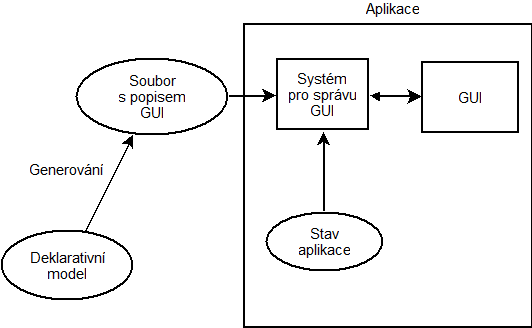
\includegraphics[width=0.7\textwidth]{modelUse}
\caption{{\label{fig:modelUse}}Diagram aplikace s používající popis GUI vygenerovaný z modelu.}
\end{center}
\end{figure*}

\section{\label{SEC:editGUI}\textit{GUI} Editory}
K návrhu a tvorbě \textit{GUI} se používají mimo jiné i speciální editory, z nichž některé umožňují i spuštění a testování navrhovaného rozhraní. Výstupem velké části takovýchto editorů bývá zpravidla kód, nějakého jazyka, který popisuje dané rozhraní, které vývojář v rámci editoru navrhl. Většina editorů umožňuje návrh rozhraní pomocí postupného vkládání elementů na kreslící plochu ze seznamu poskytovaných prvků a následně přiřazovat funkce či objekty, pro obsluhu událostí v rámci daného \textit{GUI}.\\
Některé editory bývají integrovány přímo do prostředí pro vývoj aplikací, například editor wxSmith pro vývojové prostředí \textit{Code::Blocks} pro jazyk \textit{C++}, či editor \textit{GUI} ve vývojovém \textit{NetBeans} pro jazyk \textit{Java}. V takových případech bývá vývojové prostředí použito pro současný vývoj aplikační logiky i grafického uživatelského rozhranní. Zpravidla je pak výstupem \textit{GUI} editoru kód, který je obdobný tomu, pokud by programátor naprogramoval při použití imperativního přístupu pro tvorbu \textit{GUI}.

\begin{description}
\item [wxSmith] –\textit{wxSmith} je zásuvný modul pro vývojové prostředí \textit{Code::Blocks}. Slouží k vývoji grafického rozhraní s použitím grafických elementů poskytovaných knihovnou wxWidgets pro jazyk \textit{C++}. \cite{bib:wxSmith}
\item [Swing GUI Builder] – \textit{Swing GUI Builder}, také označovaný jako \textit{Project Matisse}, je integrován do vývojového prostředí \textit{NetBeans} pro jazyk \textit{Java}.  \textit{GUI} vytvořené tímto editorem využívá funkčnost a elementy poskytované knihovnou Swing. Jeho součástí jsou i vizuální nástroje pro ladění, které umožňují během ladění aplikace uložit aktuální stav \textit{GUI} v daném momentě, přičemž uživatel pak může prozkoumávat \textit{GUI} v uchovaném stavu. Je umožněno zobrazit vlastnosti jednotlivých \textit{GUI} elementů, jejich zdrojový kód i pracovat s událostmi a třídami pro jejich obsluhu. \cite{bib:swingBuilder}
\item[Ultimate++] - \textit{Ultimate++} je vývojové prostředí pro vývoj \textit{GUI} aplikací v jazyce \textit{C++}. Jeho součástí je editor pro návrh \textit{GUI}. Toto prostředí poskytuje vlastní knihovnu se sadou několika desítek použitelných elementů. \cite{bib:ultimate}
%Qt Creator  - viz. /ref{}
\end{description}

% \ref{wxSmith} References 1
%// http://wiki.codeblocks.org/index.php?title=WxSmith_plugin 
 %\ref{swingBuilder} References 1
%// https://netbeans.org/kb/docs/java/debug-visual.html
 %\ref{Ultimate} References 1
%// http://ultimatepp.org/www$uppweb$overview$en-us.html

\section{\label{SEC:declGUI}Deklarativní \textit{GUI}}
Pro tvorbu \textit{GUI} se také používají deklarativní jazyky, tyto jazyky se zpravidla označují jako \textit{User unterface mark-up languages}. Tyto jazyky slouží pro popis uživatelského rozhraní podobně, jako například jazyk \textit{HTML} slouží pro popis dokumentu. V jazyce je zapsán popis uživatelského rozhraní, podle kterého je dané uživatelské rozhraní vytvořeno. Ve velké části případů je kód v daném jazyku interpretován za běhu aplikace systémem pro správu \textit{GUI}. Některé jazyky, mezi něž patří například \textit{QML}, lze přeložit do byte-kódu, který je v rámci cílové aplikace interpretován.\\
Následují příklady deklarativních jazyků pro tvorbu \textit{GUI}:

\begin{itemize}
\item UIML – Jedná se o jeden z prvních jazyků pro deklarativní popis uživatelského rozhraní. \textit{User Interface Markup Language} je odvozena z jazyka \textit{XML}. Jedná se o jazyk vyvinutý za účelem vytvoření univerzálního jazyka, který by mohl být použit pro tvorbu \textit{GUI} nezávisle na platformě. \cite{bib:UIML}
\item XAML – \textit{XAML} vychází z jazyka \textit{XML}. Používá se pro tvorbu \textit{GUI} aplikací v prostředí \textit{.NET}. V \textit{XAML} deklarované elementy \textit{GUI} přímo reprezentují instance jednotlivých objektů. Tento jazyk je tak silně provázán s typovým systémem prostředí \textit{.NET}. \cite{bib:XAML}
\item FXML – \textit{FXML} skriptovací jazyk vycházející z \textit{XML}. Umožňující tvořit objektové grafy v jazyce \textit{Java}. Používá se primárně pro deklaraci \textit{GUI} pro JavaFX aplikace.\cite{bib:FXML}
\item MXML – Jedná se o dalčí \textit{XML} jazyk. Je inspirován jazykem \textit{HTML}. Umožňuje zkompilování souborů do \textit{SWF} souborů. Vytvořené \textit{GUI} pak může být používáno s pomocí přehrávače jazyka \textit{Flash}. Tento jazyk umožňuje rozšíření souboru poskytovaných komponent o další, ke kterým může být přistupováno stejným způsobem.\cite{bib:MXML}
\end{itemize}

% \ref{UIML} References 1
%// http://www.ramb.ethz.ch/CDstore/www8/data/2170/pdf/pd1.pdf
% \ref{XAML} References 1
%// https://msdn.microsoft.com/en-us/library/ms752059.aspx
% \ref{FXML} References 1
%// http://fxexperience.com/wp-content/uploads/2011/08/Introducing-FXML.pdf
% \ref{MXML} References 1
%// http://help.adobe.com/en_US/flex/using/WS2db454920e96a9e51e63e3d11c0bf5f39f-7fff.html

\section{\label{SEC:QML}Jazyk \textit{QML}}
\subsection{Qt}
\textit{Qt} je multi-platformní open-source knihovna sloužící k vývoji především \textit{GUI} aplikací v jazyce \textit{C++}. Aplikace se vyznačují tzv. nativním vzhledem \textit{GUI}, což znamená, že se pro grafické rozhraní využívá standardní vzhled \textit{GUI} poskytovaný operačním systémem. Tímto je dosaženo obdobného vzhledu, jaký mají standardní aplikace pro daný operační systém. Součástí \textit{Qt} je \textit{Qt Quick}, což je soubor technologií sloužících k tvorbě deklarativního \textit{GUI}.\\
\textit{Qt} poskytuje vývojové prostředí \textit{Qt Creator}, které lze použít pro vývoj \textit{C++} aplikací využívající prvky \textit{Qt} nebo aplikací \textit{Qt Quick}. Součástí Qt creator je vizuální debuger \textit{C++}, editor kódu, grafický editor pro uživatelské rozhraní, interpret pro jazyk \textit{QML} a debugger pro jazyk \textit{QML}.

\subsection{Qt Quick}
\textit{Qt Quick} je soubor technologií sloužících k tvorbě deklarativního \textit{GUI}. Poskytuje sadu \textit{GUI} elementů, deklarativní jazyk \textit{QML} a modul \textit{Qt declarative}. \textit{Qt declarative} slouží jako modul pro využití \textit{QML} v \textit{C/C++} aplikacích, který za běhu rozparsuje vstup ve formátu \textit{QML} a sestaví podle něj \textit{GUI} s využitím funkčnosti poskytovanou Qt. Jeho součástí je interpret jazyka \textit{JavaScript}, který umožňuje evaluaci \textit{JavaScript} kódu ve funkcích definovaných v \textit{QML} souboru. \textit{Qt declarative} odděluje správu \textit{GUI} od aplikační logiky \textit{C++}. K datům vytvořených v \textit{QML} lze přistupovat v \textit{C++} části aplikace a naopak prostřednictvím tohoto modulu.

\subsection{QML}
\textit{QML} je jazyk vycházející z jazyka \textit{JavaScript}. Jedná se o jazyk pro deklaraci hierarchického \textit{GUI}, na vrcholu hierarchie je vždy jediný element a všechny ostatní elementy jsou na něj navázány ve stromové struktuře. Každý element může mít teoreticky neomezené množství potomků (elementy, jež se nacházejí v hierarchii přímo pod ním), avšak může mít nanejvýš jednoho rodiče (element, který se nachází v hierarchii přímo nad ním). Pouze kořenový element na vrcholu hierarchie nemá žádného rodiče.

\subsubsection{Syntaxe}
Základní syntaxe je ilustrována viz. Fragment kódu \ref{lst:qml1}.
\begin{lstlisting}[frame=single,caption=Tvorba dvou jednoduchých elementů pomocí jazyka \textit{QML}.,label=Tvorba dvou jednoduchých elementů pomocí jazyka \textit{QML}.,label=lst:qml1]
Rectangle
{
	width : 100; height : 100
	Image
	{
		source : "img.jpg"
	}
}
\end{lstlisting}
Soubor s tímto kódem vytvoří dva \textit{GUI} elementy. Kořenovým prvkem je element typu \textit{Rectangle}, jehož potomkem je element typu Image. Element typu Rectangle má přiřazenu hodnotu dvěma atributům width a height, zatímco element typu \textit{Image} má nastaven atribut source řetězcem "img.jpg".

\subsubsection{Přidávání nových atributů}
QML umožňuje rozšířit existující typ elementu o přídavné atributy, pomocí klíčového slova property a zadáním  datového typu atributu viz. fragment kódu \ref{lst:qml2}.
\begin{lstlisting}[frame=single,caption=Ukázka deklarace dvou nových atributů.,label=lst:qml2]
Rectangle
{
	property int newProp01
	property int newProp02 : 5
}
\end{lstlisting}
Tento kód vytvoří dva nové atributy typu int jménem \textit{newProp01} a \textit{newProp02}, přičemž \textit{newProp02} inicializuje na hodnotu $5$.
\subsubsection{Výrazy}
Hodnoty jednotlivých atributů lze definovat pomocí výrazů. Hodnoty výrazů se přepočítávají za běhu aplikace, pokud se jejich hodnota může změnit, jak je ilustrováno viz. fragmenty kódu \ref{lst:qml31},\ref{lst:qml32} a \ref{lst:qml33}.
\begin{lstlisting}[frame=single,caption=Výraz ilustrující přiřazení konstanty.,label=lst:qml31]
	width : 5
\end{lstlisting}
\begin{lstlisting}[frame=single,caption=Výraz ilustrující přiřazení hodnoty jiného atributu.,label=lst:qml32]
	width : height/2
\end{lstlisting}
\begin{lstlisting}[frame=single,caption=Výraz ilustrující přiřazení hodnoty atributu jiného elementu.,label=lst:qml33]
	width : parent.width/3
\end{lstlisting}
V prvním výrazu (\ref{lst:qml31}) je hodnota nastavena na konstantní hodnotu $5$.\\
V druhém výrazu (\ref{lst:qml31}) je atribut nastaven pomocí jiného atributu \textit{height}, kdykoli se tudíž za běhu programu změní hodnota atributu \textit{height}, pak se změní i hodnota atributu \textit{width}.\\
V posledním výrazu (\ref{lst:qml31}) je použito klíčové slovo \textit{parent}, pomocí nějž lze přistupovat k atributům nadřazeného elementu v hierarchii (tzv. rodiče). Pokud se v takovémto případě změní hodnota rodičova atributu \textit{width}, dojde i k opětovnému spočtení výrazu a tak i k úpravě hodnoty \textit{width} potomka. Tímto způsobem je umožněno dynamicky přizpůsobovat velikost i jiné atributy elementů v hierarchii v závislosti na změnách atributů jiných elementů.\\
Toto je jednou z důležitých vlastností při použití \textit{QML} k definici uživatelského rozhraní. Je tak možné provázat mezi sebou jednotlivé atributy (tzv. "property binding") tak, že se za běhu programu budou jejich hodnoty dynamicky přepočítávat kdykoli, se změní hodnoty atributů, na nichž jsou závislé .

\subsubsection{Identifikátory objektů}
Každý objekt může mít přiřazen unikátní identifikátor, pomocí nějž může být k němu přistupováno.  K tomu slouží speciální atribut \textit{id}, do nějž může být přiřazen daný identifikátor. Identifikátor musí být unikátní v dané komponontě. V Fragment kódu \ref{lst:qml4} je ukázka použití tohoho atributu.
\begin{lstlisting}[frame=single,caption=Ukázka použití atributu id.,label=lst:qml4]
Rectangle
{
	id : identifier01
	width : 100
}
Rectangle
{
	width : identifier01.width
}
\end{lstlisting}
V tomto případě je hornímu elementu nastaven atribut width na hodnotu 100 a atribut width spodního elementu je nastaven na totožnou hodnotu.

\subsubsection{Komponenty}
\textit{GUI} definované uvnitř jednoho \textit{QML} souboru se označuje jako komponenta. Každou komponentu je možné znovu použít jako stavební elemnty jiných komponent, obdobně jako je tomu u standardních typů elementů. Komponenty se importují automaticky, při použití jména souboru jako typu \textit{GUI} elementu.

\begin{lstlisting}[frame=single,caption=Ukázka použití komponenty z jiného souboru.,label=lst:qml5]
Rectangle
{
	CustomButton {}
}
\end{lstlisting}
Například existuje-li soubor "CustomButton.qml", pak kód Fragment kódu \ref{lst:qml5} vytvoří uvnitř obdélníka komponentu definovanou v importovaném souboru "CustomButton.qml".

\subsubsection{Funkce}

V \textit{QML} lze pomocí klíčového slova function definovat funkci se zdrojovým kódem v jazyce \textit{JavaScript}, při vyhodnocování výrazu v takovýchto funkcích platí totožná pravidla s těmi pro vyhodnocování výrazů přiřazených atributům.\\
Pokud místo výrazu je atributu přiřazen kód těla funkce v jazyce \textit{JavaScript} ohraničený složenými závorky, bude pro vyhodnocení hodnoty atributu použita tato funkce, výsledná hodnota atributu se v takovém případě vrací pomocí klíčového slova return.

\subsubsection{Kontrola atributů}
Kontrola existence atributů nebo kontrola datových typů je částečně řešena při zpracování \textit{QML} souboru a částečně až za běhu výsledného programu. Pokud je nějakému atributu přiřazena hodnota, je kontrolována existence daného atributu již při zpracování \textit{QML} souboru. V případech, že nelze předem určit existenci nějakého atributu (například při přístupu k atributům elementu prostřednictvím obecné reference), provádí se daná kontrola až za běhu programu.
\begin{lstlisting}[frame=single,caption=Ukázka použití komponenty z jiného souboru.,label=lst:qml6]
{
	v : w.x + d
}
\end{lstlisting}
Uvažujme příklad Fragment kódu \ref{lst:qml6} Pokud element nemá atribut se jménem \textit{v}, nastane chyba už při zpracování \textit{QML} souboru. V opačném případě mohou nastat chyby až během spuštění programu. Aby byl kód validní, musí existovat buď element identifikátorem \textit{w}, mající atribut \textit{x} typu kompatibilním s \textit{v} nebo musí element mít atribut \textit{w}, který obsahuje objekt, jež má atribut \textit{x} typově kompatibilní s \textit{v}. Zároveň musí existovat atribut \textit{d}, který je typově kompatibilní s \textit{v}, přičemž musí tento typ podporovat operaci sčítání.\\
V případě, že existuje zároveň atribut \textit{w} a element s identifikátorem \textit{w}, bere se v potaz pouze element s identifikátorem \textit{w}. Tudíž pokud existuje atribut \textit{w} obsahující atribut \textit{x}, ale zároveň existuje nějaký element s identifikátorem \textit{w}, který neobsahuje atribut \textit{x}, dojde k chybě, kvůli neexistenci atributu \textit{x} v elementu \textit{w}. 

\subsubsection{Výhody a Nevýhody}
Výhody:
\begin{itemize}
  \item Umožňuje rychlé prototypování a rychlé iterace návrh-zobrazení při tvorbě \textit{GUI}.
  \item Poskytuje velké množství \textit{GUI} elementů.
  \item Umožňuje tvorbu nových \textit{GUI} elementů, které mohou i nemusí vycházet z již poskytnutých.
  \item Multiplatfomní podpora.
  \item Umožňuje jednoduše dynamicky provázat vlastnosti různých elementů pomocí tzv. property binding.
\end{itemize}
Nevýhody:
\begin{itemize}
  \item Jedná se o interpretovaný jazyk, což znamená, že dosahuje nižšího výkonu oproti neinterpretovaným jazykům, které se kompilují do nativního kódu.
  \item Jedná se o slabě typovaný jazyk, tudíž se typy proměnných a hodnot určují až za běhu aplikace, což představuje výkonostní nevýhodu oproti silně typovaným jazykům.
\end{itemize}







\chapter{\label{CH:CQMLDes}Návrh Jazyka}
\section{\label{SEC:CQML}Jazyk \textit{CQML} - Návrh a vlastnosti}
Cílem při návrhu jazyka \textit{CQML} bylo zachovat, co největší podobnost s \textit{QML}, co se týče jeho funkčnosti a možností, ale zároveň umožnit, jednoduchou integraci do aplikací v jazyce \textit{C++}. Pro výstupní jazyk překladače byl vybrán jazyk \textit{C}. Pro jednodušší převod do výstupního formátu je pro kódy funkcí pro obsluhu událostí a výpočtů hodnot atributů oproti jazyku \textit{QML} (využívající \textit{JavaScript}) použita syntaxe jazyka \textit{C}. Což umožní ve výsledném kódu vygenerovaným překladačem například zavolání funkcí či přistupovat ke globálním proměnným.\\
Syntaxe byla zvolena podobná jazyku \textit{QML}. Rozdílem je ukončující znak středníku na konci každého výrazu. Ačkoli ukončovací znak není nutný (viz. \textit{QML} a \textit{JavaScript}), je tímto dosaženo toho, že výsledná gramatika bude nevypouštěcí, což bude mít za následek jednodušší zpracování \textit{CQML} kódu a také přesnější chybová hlášení při syntaktické analýze. Základní syntaxe je ilustrována viz. \ref{lst:cqml1}
\begin{lstlisting}[frame=single,caption=Tvorba dvou jednoduchých elementů pomocí jazyka \textit{CQML}.,label=lst:cqml1]
Rectangle
{
	id : identifier01;
	width : 100;
};
Rectangle
{
	width : identifier01.width;
};
\end{lstlisting}
Tímto způsobem se vytvoří stejné \textit{GUI}, jako v případě jazyka \textit{QML} viz. Fragment kódu \ref{lst:qml1}.\\
Podobně jako v \textit{QML}, \textit{GUI} komponenty definované uživatelem mohou být uloženy v oddělených souborech a následně importovány a opětovně používány jako samostatné elementy v jiných \textit{GUI} komponentech. Na rozdíl od \textit{QML} se soubory nebudou importovat automaticky, ale začátku každého \textit{CQML} souboru budou definovány soubory, z nichž budou importovány \textit{GUI} hierarchie a také identifikátor, jehož použitím jako typ elementu bude na dané místo umístěna importovaná komponenta. Fragment kódu \ref{lst:cqml2} ilustruje import komponenty v jazyce \textit{CQML} ze souboru "CustomButton.cqml", ke které se následně přistupuje pomocí klíčového slova \textit{Button}.
\begin{lstlisting}[frame=single,caption=Ukázka importu komponenty v jazyce \textit{CQML}.,label=lst:cqml2]
import "CustomButton.cqml' as Button;
Rectangle
{
	Button {};
}
\end{lstlisting}
Programovací jazyky zpravidla nebývají bezkontextové, nicméně jejich syntaktická analýza (nikoli však sémantická) lze provést pomocí bezkontextové gramatiky. Toto platí například pro jazyk \textit{C}, z jehož gramatiky se bude vycházet pro syntaktickou analýzu kódu funkcí a výrazů v \textit{CQML}. Z tohoto hlediska bude i gramatika \textit{CQML} bezkontextová, protože typová kontrola a kontrola existence atributů či identifikátorů nebude prováděna během syntaktické analýzy. To má za výhodu, že nebude během syntaktické analýzy potřeba použití vyhledávací tabulky pro kontrolu symbolů.\\
Pro gramatiku \textit{CQML} byla zvolena \textit{YACC} notace, vzhledem k dostupnosti technologií pro generování parseru a existenci gramatiky pro jazyk \textit{C} ve formátu \textit{YACC}. Gramatika ve formátu \textit{YACC} se nachází v příloze A \ref{CH:APA}.\\
Gramatika jazyka \textit{CQML} je víceznačná, protože pro definici funkcí a výrazů používá syntaxi jazyka \textit{C}, jehož gramatika je víceznačná. Víceznačnost je způsobena pravidlem pro podmínku \textit{IF-ELSE} (viz. Fragment kódu \ref{lst:i$f_1$}), jedná se o tzv. "dangling else problem".\\
\begin{lstlisting}[frame=single,caption=Víceznačné \textit{IF-ELSE} pravidlo gramatiky.,label=lst:i$f_1$]
selection_statement
	: IF '(' expression ')' statement
	| IF '(' expression ')' statement ELSE statement 
\end{lstlisting}
Výrok uvedený ve Fragmentu kódu \ref{lst:i$f_2$} může být podle daného pravidla rozparsován dvěma způsoby viz. Fragment kódu \ref{lst:if3}.
\begin{lstlisting}[frame=single,caption=Příklad víceznačného výroku \textit{IF}-\textit{ELSE},label=lst:i$f_2$]
if (a) if (b) s; else s2;
\end{lstlisting}

\begin{lstlisting}[frame=single,caption=Možnosti interpretace víceznačného výroku IF-ELSE,label=lst:if3]
1.
if(a){
	if(b)
		s;
	else
		s2;
}


2.
if(a){
	if(b)
		s;
}
else
	s2;
\end{lstlisting}
Podle konvencí se preferuje první způsob interpretace, který lze chápat tak, že se \textit{ELSE} přiřadí k nejvnitřnějšímu \textit{IF}.


\chapter{\label{CH:appDesign}Návrh aplikace}
Dalším cílem této práce je vytvořit nástroje, které umožní z deklarace uživatelského rozhraní v jazyce \textit{CQML} vytvořit zdrojový kód v jazyce \textit{C++}, jenž bude moci být následně využit uvnitř grafické aplikace, která deklarované uživatelské rozhraní zobrazí a umožní uživateli s ním interagovat. Vytvoření zdrojového kódu \textit{C++} bude realizováno pomocí překladače. Pro co nejjednoduší integraci vygenerovaného zdrojového kódu do uživatelské aplikace, bude vytvořena knihovna, která se bude starat o správu a vykreslování struktur vygenerované hierarchie uživatelského rozhraní. 
Na obrázku \ref{fig:structure1} je náčrtek, ukazující jednotlivé bloky, systému pro vytvoření \textit{GUI} pomocí \textit{CQML}, včetně uživatelské aplikace.  

\begin{figure*}[!ht]
\begin{center}
  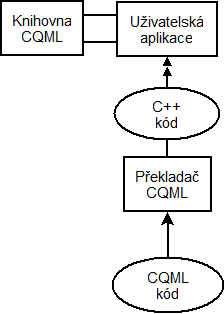
\includegraphics[width=0.7\textwidth]{Diagram1}
\caption{{\label{fig:structure1}}Návrh struktury aplikace.}
\end{center}
\end{figure*}

Jedním z cílů této práce je umožnit jednoduchou rozšiřitelnost základní funkčnosti této knihovny, například přidáním dalších \textit{GUI} elementů, které nebudou vycházet z funkčnosti již existujících, tudíž by to nebylo možné pouze jejich tvorbou pomocí \textit{CQML} souborů. Prvky, které nejsou vytvořeny pomocí \textit{CQML} souborů z již existujících prvků, se v budou nazývat vestavěné prvky.
Použití nových vestavěných typů vyžaduje jejich deklaraci v hlavičkovém souboru používaném jak v aplikaci používající knihovnu, tak i v knihovně samotné, přičemž je také nutné, aby o jejich existenci a členech věděla i aplikace překladače \textit{CQML}. Aby byla rozšiřitelnost co nejjednodušší, je potřeba, aby deklarace nových prvků musela být na co nejmenším počtu míst. Z tohoto důvodu se bude deklarace nových vestavěných prvků spolu s jejich registrací pro potřeby překladače realizovat pomocí maker v jednom souboru, přičemž funkčnost těchto maker bude v jednotlivých aplikacích rozlišena pomocí konstruktů \#ifdef.
Pro usnadnění rozšiřitelnosti budou některé metody nových vestavěných prvků vygenerovány, jako například metody pro inicializaci nebo update hodnot atributů daného typu. Generování některých takovýchto metod nemusí být triviální problém, který by šlo vyřešit pomocí maker v rámci \textit{C/C++} preprocesoru. Z tohoto důvodu je nutné přidat aplikaci, která předzpracuje vestavěné typy a vypíše zdrojové kódy vygenerovaných metod, které budou použity v rámci knihovny.

\begin{figure*}[!ht]
\begin{center}
  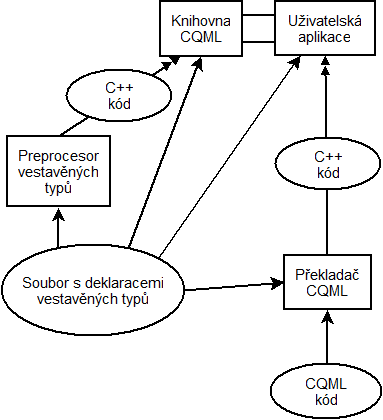
\includegraphics[width=0.7\textwidth]{Diagram2}
\caption{{\label{fig:structure2}}Návrh struktury aplikace rozšířený o části pro předzpracování datových typů.}
\end{center}
\end{figure*}

Na obrázku \ref{fig:structure2} je ilustrován finální návrh struktury systému pro vývoj \textit{GUI} v jazyce \textit{CQML}. Dvojité šipky představují vztah mezi jednotlivými bloky, kde na počátku šipky je blok, na jehož výstupu je zdrojový kód, zatímco na konci šipky je blok, do kterého je zdrojový kód zahrnut. Jednoduché šipky ilustrují, do kterých bloků bude zahrnut soubor s deklaracemi vestavěných typů nebo vstup vstup \textit{CQML} souborů.

\section{\label{SEC:macN}Deklarace vestavěných typů}
Jak již bylo zmíněno, deklarace nových vestavěných typů bude probíhat pomocí maker v jednom souboru. Funkčnost se bude lišit v závislosti na aplikaci, do které bude soubor zahrnut. V případě knihovny a uživatelské aplikace daná makra vygenerují pouze kód definující struktury nových datových typů. V případě překladače a preprocesoru vestavěných typů budou pomocí těchto maker volány funkce pro registraci nových datových typů spolu s funkcemi pro registraci jejich atributů. Ovšem k vygenerování kódu pomocí makra je nutné nejen makro vytvořit, ale i zajistit, že bude někdy provedeno, proto zde bude i jednoduchý seznam maker, která se mají provést. Pro účely preprocesoru a překladače bude potřeba i zaregistrovat primitivní typy, které budou moci být používány v rámci jazyka \textit{CQML}, proto se v seznamu prováděných maker budou nacházet i makra pro registraci primitivních datových typů. Tato makra neprovedou nic v případě knihovny \textit{CQML} či uživatelské aplikace, avšak v případě preprocesoru a překladače zavolají funkce pro registraci primitivního datového typu.

\begin{lstlisting}[frame=single,caption=Makro registrující datový typ\, v případě\, že je definováno jiné makro. ,label=lst:decprimN]
#ifdef REGISTRATION_APP
#define REGISTER_PRIMTYPE(x) RegisterPrimitive(x)
#else
#define REGISTER_PRIMTYPE(x)
#endif
\end{lstlisting}
Ve fragmentu kódu \ref{lst:decprimN} je ukázka makra, které by zavolalo funkci \textit{RegisterPrimitive} s parametrem \textit{x}, když je \textit{REGISTRATION\_APP} definováno, přičemž neprovede nic, když \textit{REGISTRATION\_APP} definováno není.


\begin{lstlisting}[frame=single,caption=Makro\, které registruje strukturu nebo vypíše její deklaraci\, v závislosti na jiném makru. ,label=lst:decN]
#ifdef REGISTRATION_APP
#define REGISTER_STRUCTURE(macro, name) \
struct name { macro(DECL_ATTRIB) };
#else
#define REGISTER_STRUCTURE(macro, name) \
RegisterStructure(name);\
macro(REG_ATTRIB) 
#endif

#define DECL_ATTRIB(type, name) type name;

#define REG_ATTRIB(type, name) RegisterAttribute(type,name);
\end{lstlisting}
  
Fragment kódu \ref{lst:decN} ilustruje makra, která by mohla být použita pro registraci struktury v jedné aplikaci, kde je \textit{REGISTRATION\_APP} definováno, a zároveň by definovali strukturu tam, kde \textit{REGISTRATION\_APP} definováno není. Fragment kódu \ref{lst:decUse1N} pak ukazuje příklad použití maker, zatímco fragment \ref{lst:decUse2N} ukazuje vygenerovaný makry kód pro případ, že je \textit{REGISTRATION\_APP} definováno, a fragment \ref{lst:decUse3N} pro případ opačný. Uživatel tak bude moci takovýmto způsobem přidat nový datový typ vytvořením makra pro vygenerování dané datové struktury a vložením názvu makra do seznamu prováděných maker.

\begin{lstlisting}[frame=single,caption=Ukázka makra\, které vytvoří/zaregistruje určitou strukturu. ,label=lst:decUse1N]
#define STRUCT_CUSTOM(OPERATION) \
OPERATION(int, first) \
OPERATION(char, second) \

REGISTER_PRIMTYPE(char)
REGISTER_PRIMTYPE(int)
REGISTER_STRUCTURE(STRUCT_CUSTOM,Custom)
\end{lstlisting}

\begin{lstlisting}[frame=single,caption=Kód vygenerovaný makrem\, který zaregistruje strukturu.,label=lst:decUse2N]
RegisterPrimitive(char);
RegisterPrimitive(int);

RegisterStructure(Custom);
RegisterAttribute(int, first);
RegisterAttribute(char, second);
\end{lstlisting}

\begin{lstlisting}[frame=single,caption=Deklarace struktury vygenerovaná pomocí makra.,label=lst:decUse3N]
struct Custom { int first; char second; };
\end{lstlisting}
 







\section{Překladač}
Cílem je vytvořit aplikaci překladače, která přemění kód z jazyka \textit{CQML} pro deklarativní \textit{GUI}, kód importovatelný do aplikace v jazyce \textit{C++}. Tudíž na vstupu bude soubor se zdrojovým kódem v jazyce \textit{CQML} a výstupem bude zdrojový kód v jazyce \textit{C++}, ve formě definicí datových struktur pro \textit{GUI} a funkcí. \\
%Vzhledem k tomu, že jazyk C na rozdíl od vyšších programovacích jazyků (C++, Java) nepodporuje členské metody u struktur (resp. tříd), je tento nedostatek %obejit tím, že se použije funkce, která je rozšířena o jeden parametr, jako který přijímá ukazatel na objekt, který by danou metodu volal. V případě virtuálních %metod je jako člen struktury použit ukazatel na funkci, která se bude volat.
Výsledný překladač je navržen tak, že lze rozdělit do několika bloků, viz. Obrázek \ref{fig:fig1}.\\
\begin{figure*}[!ht]
\begin{center}
  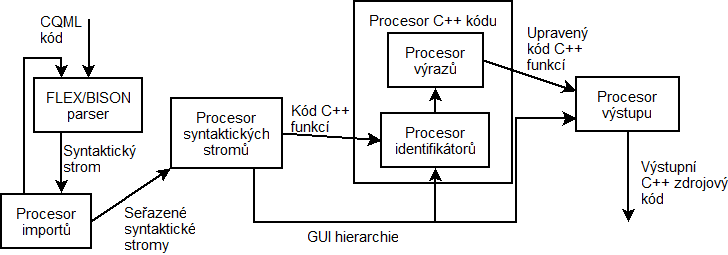
\includegraphics[width=0.7\textwidth]{parserdiag}
\caption{{\label{fig:fig1}}Návrh struktury překladače.}
\end{center}
\end{figure*}
Cílem prvního bloku (FLEX/BISON Parser) je přečíst zdrojový kód z \textit{CQML} souboru a ověřit jeho syntaktickou správnost. V případě, že je kód syntakticky v pořádku, bude výstupem tohoto bloku syntaktický strom. Pro tento blok budou použity zdrojové kódy vygenerované pomocí aplikací \textit{Bison} a \textit{Flex}, z \textit{YACC} gramatiky pro \textit{CQML}.\\
V syntaktickém stromu budou nalezeny příkazy pro import souborů (blok Procesor importů). Tyto soubory budou následně otevřeny a postupně zpracovány totožným způsobem.\\
Jakmile jsou všechny importované soubory zpracovány a jsou jejich zpracováním vytvořeny jejich syntaktické stromy, bude zjištěno, zda jsou některé soubory cyklicky závislé. To se bude realizovat pomocí konstrukce orientovaného grafu, kde každý vrchol představuje soubor a závislost mezi soubory je znázorněna hranou (směřující k importovanému souboru), a následným zjištěním zda v grafu existuje orientovaný cyklus. Pokud v grafu takový cyklus existuje, pak jsou soubory cyklicky závislé, což vyústí v chybu a ukončení programu. Je-li graf acyklický, jsou podle něho topologicky seřazeny syntaktické stromy jednotlivých souborů (vrcholy) pro následné zpracování.\\
V dalším bloku (Procesor syntaktických stromů) se zpracuje syntaktický strom a podle něj se vytvoří \textit{GUI} hierarchie. Pro každý uzel představující \textit{GUI} element, atribut, funkci, či nový atribut se vytvoří instance příslušné třídy. Každému elementu jsou podle jeho potomků v syntaktickém stromu přiřazeny jeho potomci v \textit{GUI} hierarchii a jeho atributy a funkce.
Následně se zpracují všechny elementy s definovaným atributem \textit{id}, a tyto identifikátory se použijí ke tvorbě mapy, pomocí níž bude umožněno přistupovat k danému elementu podle definovaného identifikátoru.\\
V další části programu (Procesor \textit{C++} kódu) se zpracují kódy funkcí do formy potřebné pro závěrečný výstup v jazyce \textit{C}.

\subsection{\label{SEC:tokens}Zpracování kódu v jazyce \textit{C++}}
Syntaktické stromy jednotlivých funkcí (případně výrazů) se projdou a převedou se na pole samostatných symbolů (tokenů), takovým způsobem, že jeden prvek v poli bude představovat list stromu. Vzhledem k nutnosti kontroly existence atributů, budou pro snadnější zpracování některé symboly v poli seskupeny do jednoho, který bude mít v sobě uloženo pole symbolů, které seskupil. Vzhledem k tomu, že každý symbol může obsahovat další symboly, se bude stále jednat o stromovou strukturu, nicméně, bude mít nižší hloubku.\\
\begin{figure*}[!ht]
\begin{center}
  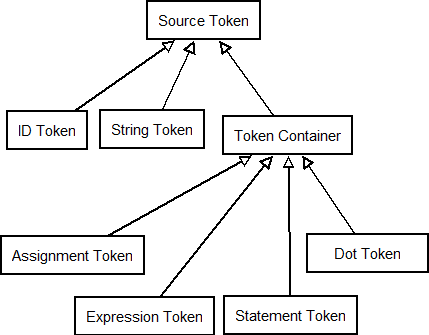
\includegraphics[width=0.7\textwidth]{tokens}
\caption{{\label{fig:fig2}}Diagram tříd symbolů.}
\end{center}
\end{figure*}

Na obrázku Obrázek \ref{fig:fig2} je znázorněn diagram tříd symbolů. Všechny třídy představující symboly dědí z jedné abstraktní třídy \textit{SourceToken}. Symboly, jež sdružují skupinu symbolů do jednoho, dědí z třídy \textit{TokenContainer}, která dědí z třídy \textit{SourceToken}. \textit{ID Token} představuje nějaký identifikátor uvnitř kodu, zatímco \textit{String Token} představuje jakýkoli jiný řetězec. \textit{Dot Token} sdružuje symboly pro výraz, v němž se pomocí operátoru "." přistupuje k atributům. \textit{Statement Token} představuje libovolný výrok, \textit{Assignment Token} představuje přiřazovací výraz a třída \textit{Expression Token} libovolný jiný výraz.

\subsubsection{Zpracování identifikátorů}
Kódy (resp. syntaktické stromy) jednotlivých funkcí se projdou, a naleznou se identifikátory, jež se nachází v mapě identifikátorů elementů (id atributy elementů), a tyto identifikátory se v kódu nahradí skutečným názvem elementu uvnitř výsledné \textit{GUI} aplikace.
\subsubsection{Dynamická kontrola typů a přiřazování hodnot}
Jelikož bude do atributů některých typů umožněno ukládat reference na objekty různého typu a pomocí této reference bude možné přistupovat k atributu daného objektu, nemůže být během kompilace určeno, že atribut, ke kterému se aplikace snaží přistoupit, je v daném objektu přítomen. Proto bude potřeba za běhu výsledné \textit{GUI} aplikace (využívající kód na výstupu překladače) kontrolovat přítomnost takového atributu.\\
Uvažujme kód \ref{lst:ref0}. Z kódu je zřejmé, že u atributu \textit{ref} bude potřeba zkontrolovat, zda má objekt referovaný tímto atributem atribut \textit{ref2} a objekt referovaný \textit{ref2} obsahuje \textit{ref3}.

\begin{lstlisting}[frame=single,caption=Pseudokód problematického použití operátoru "." v přiřazovacím výroku. \label{lst:ref0}]
width = ref1.ref2.ref3
\end{lstlisting}
Oproti nahrazení identifikátoru názvem elementu nestačí pouze nahradit část textového řetězce ve výrazu a k získání hodnoty atributu bude použita metoda \textit{Get}, která jako parametr přijímá název atributu. Kontrola bude existence atributu, je provedena uvnitř této metody a v případě, že atribut neexistuje vyhodí výjimku. Výsledný kód tak bude vypadatat, jako v ukázce kódu \ref{lst:ref1}.
\begin{lstlisting}[frame=single,caption=Řešení v pseudokódu problematického použití operátoru "." v přiřazovacím výroku. \label{lst:ref1}]
width = ref1.Get("ref2").Get("ref3");
Set("ref1",var2)
\end{lstlisting}


\subsection{Výstup}
Poslední blok se postará o výpis do výstupních souborů. Pro každý zpracovaný vstupní soubor se vytvoří hlavičkový soubor s deklarací struktur a hlaviček funkcí. Každý soubor bude mít vlastní inicializační funkci pro inicializaci hierarchie a počátečnímu přiřazení hodnot a ukazatelů na potřebné funkce.\\
Pro každý \textit{GUI} element, kterému je pomocí příkazu přidán nový atribut, se definuje nový typ struktury, která dědí z původního typu struktury. Každý přidaný atribut se deklaruje v nové struktuře, spolu s ukazatelem na funkci, která bude sloužit k jeho updatování. Pro každou takovou strukturu se také vytvoří funkce, které takovou strukturu alokují a inicializují, přičemž se v dané funkci zavolá funkce pro inicializaci struktury, ze které se dědí.\\
Pro všechny elementy se vytvoří funkce pro jejich update, která slouží k updatování hodnot v atributech elementů. Pro každý atribut, jemuž je přiřazena nějaká hodnota v \textit{CQML} souborech, bude definována funkce pro jeho update danou hodnotou. Ukazatel na danou funkci, bude přiřazena v inicializační funkci daného souboru, do členské proměnné struktury určené pro daný atribut.\\


\section{\label{SEC:prepN}Preprocesor datových typů}
Tato aplikace bude využívat výše zmíněný soubor s deklaracemi vestavěných typů, které jsou realizovány pomocí maker (viz. sekce \ref{SEC:macN}). Pro účely předzpracování datových typů v rámci preprocesoru, se pomocí maker z daného souboru zaregistrují jednotlivé vestavěné typy, spolu se seznamem jejich atributů. Také se zvlášť zaregistrují primitivní typy. Ze seznamu atributů se vygenerují hašovací funkce pro všechny vestavěné typy pomocí algoritmu popsaného v sekci \ref{SEC:hashP}.\\
Účelem preprocesoru je vygenerovat zdrojové kódy, pro použití v runtime knihovně \textit{CQML}. Vygenerují se zdrojové kódy metod pro přístup k obecnému atributu pomocí jeho jména, to k jakému atributu se bude přištupovat bude rozlišeno pomocí hodnoty haše, která je výstupem příslušné hašovací funkce. Také se vygenerují metody pro update hodnot atributů daného vestavěného typu pomocí updatovacích funkcí, které mohly být přiřazeny v rámci překladače. Dále se vygeneruje kód konstruktorů, které inicializují hodnoty atributů na jejich výchozí hodnotu, přičemž se v jejich rámci také inicializuje hodnota identifikátoru typu. Hodnota tohoto identifikátoru, který je pro každý typ unikátní, bude sloužit k výběru příslušné hašovací funkce pro daný typ v metodě pro přístup k obecnému atributu pomocí jeho jména.\\
Kód, který bude výstupem tohoto preprocesoru, bude zahrnut do kódu pro runtime knihovnu \textit{CQML}.\\


\subsection {\label{SEC:hashP} Hašování}
Hašovací funkce je zobrazení. Je-li dána množina \textit{W} slov o konečné délce skládajících se ze symbolů abecedy, pak je hašovací funkce takové zobrazení, které přiřadí každému slovu z množiny \textit{W}, právě jednu celočíselnou hodnotu z nějakého intervalu $[0,k-1]$. Pokud nějakým dvěma různým slovům z množiny W je hašovací funkcí přiřazena stejná celočíselná hodnota, pak se hovoří o tzv. kolizi.
Dokonalá hašovací funkce, je taková funkce, která pro každé slovo z dané množiny \textit{W} vygeneruje unikátní celočíselnou hodnotu v nějakém intervalu $[0,k-1]$. V takovém případě se hovoří o tzv. bezkolizní nebo dokonalé hašovací funkci. Jsou-li slova z množiny W klíči datových prvků nějaké množiny dat, pak lze mít taková data uložená v poli tak, že lze s pomocí bezkolizní hašovací funkce přímo přistupovat k jednotlivým prvkům, jelikož výsledkem takové funkce může být index do pole dat. Dané pole však by muselo mít naalokováno k prvků a to i v případech, že pro počet m skutečných datových záznamů platí $m<k$. Tudíž je jasné, že by pro ideální hašovací funkci pro tento účel platilo, že $m=k$, přičemž by tato funkce musela zůstat bezkolizní. Taková funkce se nazývá minimální dokonalá hašovací funkce.
Výhodou minimální dokonalé hašovací funkce je, že se dá použít pro efektivní uskladnění dat označených klíči. Nevýhodou je výpočetně náročné hledání takové funkce, což má za následek to, že se v praxi nedá použít pro dynamicky se měnící soubory klíčů. Tudíž se používá pouze pro statické množiny klíčů. Za další nevýhodu lze považovat, že taková funkce může mít vyšší paměťovou náročnost pro uchování svých parametrů a také může mít náročnější výpočet, i když ten bude stále asymptoticky konstantní pro konečný počet klíčů.
Aplikace bude využívat algoritmus pro nalezení dokonalé hašovací funkce z [\cite{bib:hashPerfect}], jehož výsledná hašovací funkce má tvar \ref{eq:hash1}.
Kde $f_1$ a $f_2$ jsou funkce mapující řetězec na celočíselnou hodnotu, zatímco $g$ je funkce mapující libovolné celočíselné hodnoty do rozsahu $[0,m-1]$, přičemž $m$ je počet klíčů. 
\begin{equation} \label{eq:hash1}
h(w) = (g(f_1(w))+g(f_2(w))) mod m
\end{equation}
Tento algoritmus je založen na metodě generování náhodných neorientovaných grafů. Na počátku je graf o $N$ vrcholech, přičemž jeho hrany jsou definovány tak, že každá hrana představuje jedno slovo z množiny klíčů. Výsledky funkcí $f_1$ a $f_2$, na jejichž vstupu je příslušné slovo, určují počáteční a koncový vrchol takové hrany. Je-li výsledný graf acyklický, lze najít takové ohodnocení jeho vrcholů, že součet hodnot koncových vrcholů pro každou hranu vygeneruje unikátní číslo v rozsahu $[0,m-1]$. Cílem je tedy najít funkce $f_1$ a $f_2$. Tyto funkce na vstupu přijímají slovo z množiny klíčů a na výstupu je celočíselná hodnota v rozsahu $[0,N-1]$. Vzorec \ref{eq:hash2} ukazuje takovou funkci. $T_k$ je v tomto případě jednorozměrná tabulka, která obsahuje hodnotu pro každou možnou pozici ve slově (tudíž její velikost je rovna maximální délce slova v množině klíčů), a $w[i]$ je číselná hodnota znaku slova. Tabulky $T_1$ a $T_2$ se hledají generováním náhodných čísel v rozsahu $[0,N-1]$. $N$ je nějaké zvolené číslo, které musí být větší než $m$, jinak by nebyl vygenerovaný graf nikdy acyklický. Pro příliš nízké hodnoty hrozí, že algoritmus bude trvat příliš dlouho, či nikdy neskončí, zatímco pro příliš vysoké hodnoty zabere uchovávání grafu větší místo v paměti.
\begin{equation} \label{eq:hash2}
f_k(w)=(\sum\limits_{i=1}^{|w|} T_k(i) \times w[i]) mod n
\end{equation}
\begin{equation} \label{eq:hash4}
g(v) := (h(e=(u,v))-g(u)) mod m
\end{equation}
Algoritmus se skládá ze dvou fází, mapování a přiřazení. V první fázi se vygenerují náhodně tabulky $T_1$ a $T_2$. Pomocí funkcí $f_1$ a $f_2$ se vytvoří graf výše popsaným způsobem a následně se zjistí, zda je graf acyklický, je-li tomu tak, pak se fáze opakuje, jinak se pokračuje fází přiřazení. 
 Ve fázi přiřazení se každému vrcholu grafu přiřadí hodnota, jež bude použita pro výpočet hašovací funkce. Postupně se prochází jednotlivé vrcholy. Nebyl-li nějaký vrchol \textit{u} ještě navštíven, je ohodnocen hodnotou nula a zpracují se jeho sousedé a to tak, že se jim přiřadí hodnota vypočtená podle vzorce \ref{eq:hash4}, kde $h$ vrací index slova v množině klíčů, které přísluší hraně spojující souseda \textit{v} s vrcholem \textit{u}, a $g$ je ohodnocení vrcholu. Soused je pak rekurzivně zpracován, jako byl zpracován vrchol \textit{u}.
\begin{equation} \label{eq:hash3}
h(w) = (((\sum\limits_{i=1}^{|w|} T_1(i) \times w[i]) mod n) + ((\sum\limits_{i=1}^{|w|} T_2(i) \times w[i]) mod n)) mod m
\end{equation}
Výsledná hašovací funkce je ilustrována vzorcem \ref{eq:hash3}.  Pro její uchování tedy stačí uchovat ohodnocení všech vrcholů grafu $g$ a hodnoty tabulek $T_1$ a $T_2$.



\section{\label{SEC:libI}Knihovna}
K zajištění co největší multiplatformní podpory \textit{CQML} aplikací, bude aplikace podporovat vyměnitelné externí rozhraní pro vykreslování, vstup a správu zdrojů (např. obrázky, fonty). Proto tato funkčnost nebude implementována v rámci knihovny, ale bude muset být poskytnuta v rámci uživatelské aplikace. 
Jelikož knihovna bude předkompilovaná nezávisle na uživatelské aplikaci, není možné, aby z knihovny byly přímo volány funkce v uživatelské aplikaci, protože nejsou v době kompilace knihovny ještě známy. Tudíž není možné volat například vykreslovací funkce zevnitř knihovny. Tento problém lze vyřešit předáním ukazatele na funkci v uživatelské aplikaci prostřednictvím funkce poskytované knihovnou. Vzhledem k velkému počtu vykreslovacích funkcí budou funkce sdruženy pod abstraktní třídu (interface), jako virtuální metody, které bude muset implementovat uživatelská aplikace.\\

Ve většině realtime aplikací je rozděleno vykreslování a aplikační výpočty do dvou oddělených fází, které se neprotínají. Fáze s aplikačními výpočty se zpravidla nazývá Update. Tyto fáze jsou tudíž odděleny i v případě knihovny. Během vykreslovací fáze bude vykreslována aktuální \textit{GUI} hierarchie, zatímco během fáze \textit{Update} se budou přepočítávat hodnoty uvnitř jednotlivých elementů.\\

\subsection {Vstup}
V realtime aplikacích se v některých případech bere vstup ze vstupních zařízení v odděleném vláknu, než v jakém probíhá hlavní vlánko aplikace, to má za úkol zajistit, že aplikace nezamrzne vůči uživatelově vstupu v případě, že právě provádí složitý výpočet či vykresluje složitý obraz. Proto bude knihovna podporovat tento přístup. Vstup bude zpracovávat pomocí událostí, události bude muset generovat uživatelská aplikace, která je bude prostřednictvím funkce ukládat do fronty pro jejich zpracování. Vkládat události do fronty bude umožněno i v odděleném vláknu, proto bude knihovna využívat threadsafe frontu, která bude realizována pomocí dvou oddělených front, přičemž do jedné fronty bude možno vkládat události, zatímco se druhá bude zpracovávat (viz. obrázek \ref{fig:que1N}). Zpracování fronty bude probíhat na počátku fáze \textit{Update}, jakmile se fronta zpracuje, prohodí se fronta pro vkládání událostí a pro zpracování. Fronta bude pomocí vláknových zámků zajišťovat, že při vkládání zároveň s prohozením front, nebo při vkládání událostí ze dvou vláken v tentýž okamžik, nedojde k porušení atomicity jednotlivých operací.\\
\begin{figure*}[!ht]
\begin{center}
  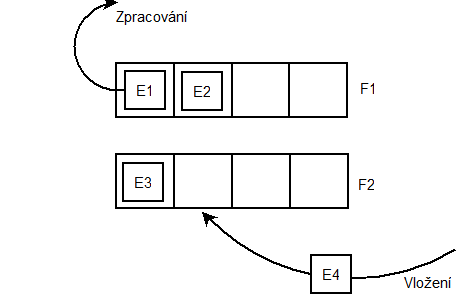
\includegraphics[width=0.7\textwidth]{Diagram5}
\caption{{\label{fig:que1N}}Návrh realizace fronty.}
\end{center}
\end{figure*}
Komunikace mezi knihovnou a uživatelskou aplikací je ilustrována na obrázku \ref{fig:lib1N}.
\begin{figure*}[!ht]
\begin{center}
  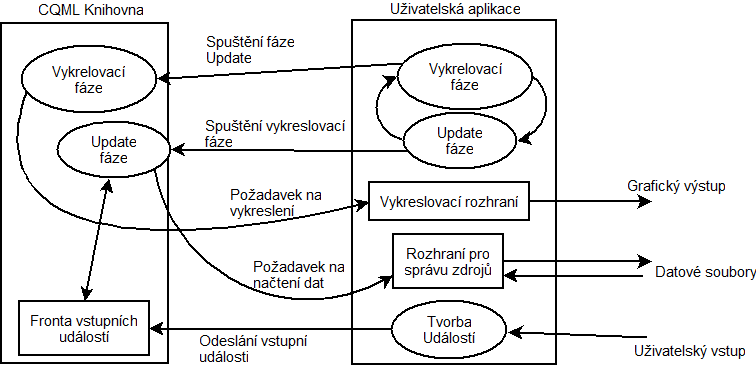
\includegraphics[width=0.7\textwidth]{Diagram4}
\caption{{\label{fig:lib1N}} Návrh komunikace mezi knihovnou a uživatelskou aplikací}
\end{center}
\end{figure*}

\subsection {Správa \textit{GUI}}
Hierarchie vygenerovaného \textit{GUI} bude uchovávána v podobě stromu. Na vrcholu stromu se tudíž nachází kořenový element, jež může mít libovolný počet potomků, přičemž každý takovýto potomek je element, který může mít opět neomezený počet potomků. Každý vestavěný datový typ, který bude přímo součástí hierachie a ne pouze atributem nějakého elementu, bude dědit z obecné struktury \textit{Element}. Každý uzel v rámci stromu \textit{GUI}, tak bude typu \textit{Element} nebo typu, který je z něj odvozen. Typ \textit{Element} bude struktura, která bude obsahovat pole jeho potomků, atributy souřadnice a velikost. Struktura \textit{Element} bude vlastnit virtuální metody Draw a Update, které budou moci struktury z nich odvozené přetěžovat.
%-- element

Každý element může mít atributy, které budou přístupné zevnitř kódu \textit{CQML}. Takové atributy uvnitř struktury reprezentující daný element, nejsou představovány pouze členem pro uchování jejich hodnoty, ale také ukazatelem na funkci, která může slouží k přepočítání hodnoty daného atributu v rámci fáze \textit{Update}. Funkce, na kterou daný ukazatel ukazuje, je vygenerována pomocí překladače a je danému atributu přiřazena. Jelikož se jedná o ukazatel na funkci a nikoliv o metodu samotného elementu, je uchováván i tzv. kontext funkce. Kontextem funkce je v tomto případě myšlen \textit{CQML} soubor v jehož rámci byla daná funkce specifikována, což znamená, že tato funkce by měla být schopna přistupovat ke všem elementům v hierarchii specifikované v daném souboru. Jelikož každý \textit{CQML} soubor představuje samostatnou komponentu, je tak kontext uložen ve formě struktury, která obsahuje ukazatel na kořenový prvek v rámci dané komponenty (souboru) a také ukazatel na element jemuž byla funkce s daným kontextem uložena.\\
%--
Každý element v \textit{GUI} hierarchii má metodu Update, kterou dědí z typu \textit{Element}. Tato metoda má za úkol přepočítat hodnoty atributů, jsou-li jim přiřazeny funkce pro jejich přepočítání. Dále tato metoda zavolá Update všech potomků daného elementu.

\subsection {Vykreslování}
Aby bylo zajištěno, že se element nacházející výše v hierarchii vždy vykreslí před elementy, jež jsou v hierarchii níže, tak se pro vykreslování použije fronta. Na počátku vykreslovací fáze se do ní zařadí pouze prvek na vrcholu hierarchie. Na prvek ve frontě se zavolá jeho vykreslovací metoda, která jej vykreslí a záriveň přidá jeho potomky na konec fronty. Po vyprázdnění fronty se ukončí fáze vykreslování.\\
Jak již bylo zmíněno, samotné vykresovací funkce budou z knihovny pouze volány pomocí vykreslovacího rozhraní poskytovaného uživatelskou aplikací. Tyto funkce budou volány zevnitř přetížených metod Draw, jednotlivých elementů. Každý vestavěný typ, který dědí z typu \textit{Element} může přetěžovat vykreslovací metodu Draw.\\
Jelikož by knihovna \textit{CQML} měla umožnit použití externích zdrojů, jako jsou například obrázky či fonty, v obecném formátu. Bude správa těchto dat obsluhována uvnitř uživatelské aplikace podobně, jako je tomu u vykreslování, pomocí speciálního rozhraní. Každý element, který taková data vyžaduje bude moci v rámci své přetížené metody Update dát do fronty požadavek pro načtení dat.\\
Tyto požadavky budou zpracovány na konci fáze \textit{Update} zavoláním příslušné metody rozhraní pro načtení dat. Metody rozhraní budou vracet hodnotu typu \textit{void*}, což může představovat ukazatel na libovolná data. Tato hodnota, pak bude uložena do mapy, pod specifickým identifikátorem, v případě obrázku bude takovým identifkátorem název souboru, v případě fontu bude tento identifikátor název fontu, který bude mít za sebou připojeny parametry fontu ve formě textového řetězce. Kdykoliv pak bude knihovna vyžadovat manipulaci s externím zdrojem (například předáním funkci pro vykreslení), učiní tak pomocí dané hodnoty typu \textit{void*}. \\
\subsection {Inicializace}
Před použitím \textit{CQML} knihovny v rámci uživatelské aplikace bude nutné knihovnu nejprve inicializovat. Během inicializace bude nutné knihovně předat ukazatele na instance objektů implementující rozhranní, jež slouží ke správě externích zdrojů a vykreslování. Také bude potřeba předat knihovně ukazatel na funkci pro inicializaci Hašovacích funkcí.\\

\subsection {Variant}
\begin{lstlisting}[frame=single,caption=Ukázka \textit{CQML} kódu ilustrující nemožnost staticky určit existenci specifického atributu.,label=lst:var01N]
Element
{
	id: firstElement;
	property Element ref:secondElement;
	witdth :   ref.status;
	MouseClick :
	{
		ref=thirdElement;
	};
};
Element
{
	id: secondElement;
	property int status : 0;
};
Element
{
	id: thirdElement;
};
\end{lstlisting}
Každý element může mít atribut v němž se uchovává reference na jiný element. Každý element může být rozšířen o atribut libovolného typu a názvu. Jelikož se za běhu programu může změnit, na který element reference ukazuje, nelze při přistupování k atributům referencovaného elementu staticky určit jejich typ ani to, zda daný element takový atribut vůbec má. Toto je problém, jelikož jazyk \textit{C/C++} je staticky typovaným jazykem, což znamená, že není možné manipulovat s hodnotou, aniž by byl v době kompilace znám její typ. Toto je ilustrováno v kódu \ref{lst:var01N}, kde se po kliknutí na první element změní, na který element reference ukazuje. Z tohoto důvodu bude k atributům takového elementu nutno přistupovat pomocí virtuální metody, která musí vracet nějaký obecný typ, do kterého může být uložena hodnota libovolného typu, se kterou bude následně možno manipulovat.\\
Pro manipulaci s hodnotami různého datového typu uniformní způsobem lze v jazyce \textit{C/C++} použít konstrukt union. Konstrukt union však nelze použít v objektově orientovaném prostředí, jelikož nepodporuje použití datových typů s netriviálním konstruktorem či destruktorem, datové typy s triviálním konstruktorem se označují zkratkou \textit{POD} ("Plain old data"), také se označují jako pasivní datové struktury.\\
Pro jazyk \textit{C/C++} existuje knihovna \textit{Boost} \cite{bib:boost}, která poskytuje řešení v podobě šablony \textit{variant}. Šablona \textit{variant} umožňuje uložení libovolného datového typu, ať už se jedná o typ \textit{POD} či nikoliv.\\
V jazyce \textit{QML} tuto funkci má datový typ \textit{var}. Tento typ má obdobnou funkci jako proměnná v jazyce \textit{JavaScript}, tudíž je do něj možné uložit data libovolného datového typu. Proměnný typ \textit{var} tak umožňuje nejen ukládání primitivních a složených datových typů, ale lze jej také použít k uložení referencí na grafické elementy. Tento typ také podporuje provádění aritmetických operací, uložení do jiné proměnné libovolného typu, přičemž pokud dojde k použití aritmetické operace mezi nekompatibilními typy (například mezi referencí na element a číselným typem), či pokusu o uložení do proměnné nekompatibilního typu, pak \textit{QML} aplikace vyhodí výjimku.\\
Pro účely knihovny \textit{CQML} je tedy vhodné vytvořit datový typ, který by se svou funkčností co nejvíce podobal typu var jazyka \textit{QML}. Tento typ bude nazýván \textit{Variant}. Pro odlišení mezi šablonou \textit{Variant} poskytovanou knihovnou boost má název tohoto typu velké počáteční písmeno.\\
Typ \textit{Variant} v knihovně \textit{CQML} bude přetěžovat operátory aritmetických operací a operátor přiřazení. Typ \textit{Variant} bude podporovat konverzi na libovolný datový typ pomocí metody \textit{As}, která bude definována pomocí šablony, jenž bude přijímat požadovaný datový typ jako parametr. Typ \textit{Variant} bude uchovávat identifikátor svého typu a svou hodnotu. Za účelem, aby se každá operace prováděla jen mezi totožnými typy, bude zavedena konvence, že při použití binárního operátoru bude vždy pravý operand přetypován na typ levého operandu. Každá konvenrze mezi typy, které nejsou kompatibilní (například mezi nečíselným a číselným typem) vyústí v chybu.\\
Typ \textit{Variant} bude podporovat metodu \textit{Get}, která v případě, že \textit{Variant} obsahuje referenci na nějaký element, umožní získat hodnotu atributu jehož název byl metodě předán jako parametr (podobně jako je tomu u složených typů používaných v rámci knihovny \textit{CQML}). V případě, že je v typu \textit{Variant} uložen primitivní typ, který nemá žádné atributy, pak dojde k ohlášení chyby, podobně jako by tomu bylo v případě žádosti o získání neexistujícího atributu.\\
\begin{lstlisting}[frame=single,caption=\textit{CQML} kód měnící hodnotu atributu elementu\, prostřednictvím reference na daný element.,label=lst:var0N]
Element
{
	id: firstElement;
	property Element ref:secondElement;
	MouseClick :
	{
		ref.status = 1;
	};
};
Element
{
	id: secondElement;
	property int status : 0;
};
\end{lstlisting}
\begin{lstlisting}[frame=single,caption=Přeložený kód funkce\, který ilustruje nutnost vrácení reference metodou \textit{Get}.,label=lst:var00N]
ref.Get("status")=1;
\end{lstlisting}
Při manipulaci s elementem pomocí reference může dojít k situaci, kdy je potřeba změnit hodnotu nějakého z jeho atributů. Tato situace je ilustrována v ukázce kódu \ref{lst:var0N}, kde po kliknutí na první element se má pomocí reference změnit hodnota atributu \textit{status} druhého elementu. Po zpracování se vnitřek funkce pro obsluhu události kliknutí, převede na kód v \ref{lst:var00N}. Problémem, který zde nastává je, že metoda \textit{Get} vrací hodnotu typu \textit{Variant}, která není nijak vázaná na adresu, kde byla původní hodnota uložena. Proto je potřeba vytvořit další datový typ, který narozdíl od typu \textit{Variant} bude namísto hodnoty uchovávat adresu atributu, kde byla původní hodnota uložena. Tento datový typ budiž nazván \textit{VariantRef}. \textit{VariantRef} bude implementovat metodu \textit{Get}, stejně jako ostatní typy používané v rámci \textit{CQML}. \textit{VariantRef} bude také přetěžovat operátor přiřazení, přičemž při použití tohoto operátoru se změní hodnota na adrese, na níž \textit{VariantRef} ukazuje. Kvůli možnosti změnit hodnotu referencovaného atributu budou tedy metody \textit{Get} všech typů v rámci \textit{CQML} (včetně \textit{VariantRef} a \textit{Variant}) vracet typ \textit{VariantRef} namísto \textit{Variant}. Jelikož typ \textit{Variant} podporuje narozdíl od \textit{VariantRef} i aritmetické operace, bude \textit{VariantRef} podporovat implicitní přetypování na typ \textit{Variant}, zkopírováním hodnoty na adrese, na níž ukazuje \textit{VariantRef}, do nové instance typu \textit{Variant}.\\


\begin{lstlisting}[frame=single,caption=Řádek \textit{CQML} kódu ilustrující přístup k atributům elementů uložených v referenci.,label=lst:var1N]
reference1.att1 = reference2.att2 = reference3.att3 + 3;
\end{lstlisting}

\begin{lstlisting}[frame=single,caption=Kód ilustrující operace s typy \textit{Variant} a \textit{VariantRef}. ,label=lst:var2N]
reference1.Get("att1") = reference2.Get("att2") = reference3.Get("att3") + 3;
\end{lstlisting}
Fragment \ref{lst:var2N} ukazuje, jak by vypadal kód funkce z fragmentu \ref{lst:var1N} po přeložení do \textit{C++}. Výsledky metod \textit{Get} jsou hodnoty typu \textit{VariantRef}, přičemž výsledek operace sčítání v daném kódu bude typu \textit{Variant}. Tato hodnota je následně uložena do attributu \textit{att1} v prvku referencovaném v \textit{reference1} a hodnota atributu \textit{att2} v prvku referencovaném v \textit{reference2}.\\


\chapter{\label{CH:Impl}Implementace}
\section{\label{SEC:header}Přidávání vestavěných typů}
Vestavěné struktury lze rozdělit na dvě různé skupiny. První skupina jsou struktury, ke kterým se bude v rámci aplikace přistupovat jako k referenčním typům, tudíž při manipulaci s nimi se manipuluje s ukazatelem ukazující na jejich umístění v paměti. Ve druhé skupině jsou struktury, které fungují jako hodnotové typy, takže se manipuluje přímo s jejich obsahem (hodnotou).\\
Zdrojový kód je sdílený mezi několika aplikacemi. Pomocí konstruktu \textit{\#ifdef CQML\_PARSER} je rozlišeno, jaké definice maker se budou v dané aplikaci používatW. Přičemž makro \textit{CQML\_PARSER} je definováno pro aplikaci překladače a preprocesoru vestavěných typů, zatímco pro grafickou knihovnu a uživatelskou aplikaci definováno není. Výstupem jsou tedy dvě verze kódu. Verze s definovaným makrem \textit{CQML\_PARSER} bude dále označována jako parser verze. Verze bez definice makra \textit{CQML\_PARSER} bude dále označována jako runtime verze.\\
Prvním makrem je makro \textit{REGISTRATION}, toto makro je jedinné voláno přímo, zatímco ostatní makra pro definici vestavěných datových typů jsou volána prostřednictvím tohoto makrem ať už přímo nebo transitivně. Makro \textit{REGISTRATION} se v parser verzi nachází uvnitř funkce RegisterBasicTypes(), která je volána na začátku aplikací překladače a preprocesoru vestavěných typ. V runtime verzi se toto makro nachází uvnitř namespace \textit{CQML}\_\textit{GUI}. Makro samotné v obou verzích má totožnou funkčnost. \textit{REGISTRATION} přijímá tři parametry, jimiž jsou makra. První je reprezentováno názvem MACRO2, které slouží pro registraci nové struktury hodnotového typu, zatímco druhým parametrem je MACRO2REF, které slouží pro registraci struktury referenčního typu. Třetím parametrem je MACRO3, což slouží pro registraci struktury dědící z jiného již registrovaného datového typu. MACRO2 a MACRO2REF přijímá jako první parametr název makra pro generování datové struktury, jako druhý parametr přijímá název datové struktury. MACRO3 má totožné první dva parametry, ale má i třetí parametr, který je názvem datového typu, ze kterého generovaná struktura dědí. \\
Na počátku makra \textit{REGISTRATION} se volají makra \textit{REGPRIMITIVE} pro primitivní datové typy, jako jsou například int, char či float. V parser verzi se pomocí makra \textit{REGPRIMITIVE} zavolá funkce RegisterPrimitive, která jako parametr přijímá název primitivního datového typu, který byl makru předán jako parametr. Makro \textit{REGPRIMITIVE} v případě runtime verze neprovede nic. Ve zbytku makra \textit{REGISTRATION} se volají makra, která mu byla předána v parametrech, s parametry pro registraci jednotlivých datových typů.\\
Makru \textit{REGISTRATION} jsou v runtime verzi předána makra \textit{MAKE\_STRUCTURE2} (toto makro je předáno jako první dva parametry) a makro \textit{MAKE\_STRUCTURE3}. Zatímco v parser verzi jsou předána makra \textit{PARSER\_DECLARE2}, \textit{PARSER\_DECLARE2REF} a \textit{PARSER\_DECLARE3}.\\
Makra \textit{MAKE\_STRUCTURE2} a \textit{MAKE\_STRUCTURE3}, mají téměř totožnou funkčnost. Vytvoří tělo struktury s definovaným názvem, konstruktorem a metodou \textit{Get} pro získání libovolného atributu. Jedinným rozdílem je, že v případě makra \textit{MAKE\_STRUCTURE3} dědí vygenerovaná struktura z typu, jehož název byl makru předán pomocí třetího parametru, zatímco struktura vygenerovaná makrem \textit{MAKE\_STRUCTURE2} dědí ze struktury \textit{CQML}Object. Makro, které bylo předáno jako první parametr, slouží k vygenerování kódu pro deklaraci atributů v těle dané struktury, pomocí maker několika maker, jež mu jsou předány jako parametry.\\
%..
Makra \textit{PARSER\_DECLARE2}, \textit{PARSER\_DECLARE2REF} a \textit{PARSER\_DECLARE3}, volají funkci, které jako první parametr předají jméno struktury (druhý parametr předaný makru) a jako druhý parametr předají nulu, v případě prvních dvou maker, a v případě třetího makra se předá jméno rodiče (třetí parametr předaný makru). První a třetí makro takto volá funkci RegisterStruct a druhé makro takto volá funkci RegisterStructRef. Všechny tři makra na závěr zavolají makro, jenž jim bylo předáno prostřednictvím prvního parametru. Volané makro slouží k zavolání funkcí pro registraci jednotlivých atributů, pomocí několika maker, jež mu jsou předány jako parametry.\\
%..
Zmíněná makra \textit{PARSER\_DECLARE2}, \textit{PARSER\_DECLARE2REF}, \textit{PARSER\_DECLARE3}, \textit{MAKE\_STRUCTURE2} a \textit{MAKE\_STRUCTURE3} příjímají jako první parametr stejný druh makra, respektive makra vycházející ze stejného vzoru. Toto makro slouží pro vygenerování deklarace atributů v runtime verzi a pro registraci atributů v parser verzi. Pro každý vestavěný typ je jedno takové makro. Makro přijímá 5 maker jako a svoje parametry v následujícím pořadí.
\begin{description}
\item[MF] slouží pro vytvoření atributu, který bude přístupný pouze ve vnitřním \textit{C++} kódu knihovny. V parser verzi toto makro zaregistruje daný atribut. V runtime verzi toto makro deklaruje atribut uvnitř struktury.
\item[F] slouží pro vytvoření atributu, který bude přístupný uvnitř \textit{CQML} souborů i ve vnitřním \textit{C++} kódu knihovny. V parser verzi toto makro zaregistruje daný atribut. V runtime verzi toto makro deklaruje atribut uvnitř knihovny, spolu s ukazatelem na funkci pro jeho výpočet a ukazatelem na kontext, v jakém bude daná funkce  operovat.
\item[M] vytvoří ukazatel na funkci, která může sloužit například k obsluze událostí. V parser verzi toto makro zaregistruje daný ukazatel. V runtime verzi toto makro deklaruje ukazatel na funkci spolu s ukazatelem na kontext, v jakém bude daná funkce operovat. 
\item[ME] deklaruje metodu, kterou bude nutno implementovat v rámci zdrojového kódu knihovny. V parser verzi toto makro neprovede nic. V runtime verzi deklaruje hlavičku metody.
\item[MEV] deklaruje virtuální metodu, kterou bude nutno implementovat v rámci zdrojového kódu knihovny. V parser verzi toto makro neprovede nic. V runtime verzi deklaruje hlavičku virtuální metody.
\end{description}
Všechna uvedená makra přijímají jako první parametr typ (v případě metod a ukazatelů na funkce je to návratový typ), jako druhý parametr název, jako třetí parametr výchozí hodnotu (tento parametr je irelevantní pro metody). Makra \textit{M}, \textit{ME} a \textit{MEV} přijímají jako zbylé parametry seznam parametrů daných funkcí (resp. metod).\\

%.. příklad


\section{\label{SEC:transImpl}Překladač}
\subsection{Zpracování vstupu}
Pomocí generátoru \textit{Bison} byl podle gramatiky jazyka \textit{CQML} vytvořen parser. Pro vygenerování lexikálního analyzátoru byl použit \textit{FLEX}. Zdrojový kód parseru a lexikálního analyzátoru je pak použit v překladači.
Po spuštění program načte výchozí typy \textit{GUI} elementů, uloží si jejich názvy a seznam jejich atributů, včetně jejich typů a výchozích hodnot, do instancí třídy \textit{ClassContainer}.\\
Program na vstupu přijímá jméno souboru, se zdrojovým kódem v jazyce \textit{CQML}. Pokud daný soubor existuje, je otevřen a jeho obsah je předán parseru. Pokud parser detekuje syntaktickou chybu ve zdrojovém souboru, vypíše chybu a program se ukončí. Výstupem parseru je syntaktický strom. V první fázi se ve stromu vyhledají příkazy pro import elementu z jiných souborů. Totéž program cyklicky provede pro všechny soubory, z nichž se elementy importují.

\subsection{Konstrukce a zpracování pomocných struktur}
Následně je vytvořen orientovaný graf vzájemných závislostí mezi jednotlivými soubory, kde každý vrchol představuje soubor a každá hrana představuje vazbu mezi soubory, zatímco počátečním vrcholem hrany je vrchol představující soubor, do něhož je element importován, a koncovým vrcholem je vrchol představující soubor, z nějž byl element importován. Pomocí algoritmu prohledávání do hloubky je zjištěno, zda se v grafu nachází cyklus. Pokud se v grafu nachází cyklus, je vypsána chybová hláška a program se ukončí.\\
Jelikož je graf acyklický, pak každý vrchol představuje komponentu a tak lze jednotlivé vrcholy grafu a tudíž i soubory topologicky seřadit. Soubory (resp. vrcholy v grafu) jsou seřazeny pomocí Tarjanova algoritmu. Syntaktické stromy jednotlivých seřazených souborů jsou postupně zpracovány následujícím způsobem.\\
Během průchodu stromem se postupně alokují instance třídy \textit{Element}, přičemž každá instance představuje určitý element v hierarchii \textit{GUI}. Každému elementu je přiřazen jeho typ a seznam jeho potomků resp. elementů, které se v hierarchii nachází níže. Dále je každému elementu, u nějž jsou definované změny některých z jejich atributů, přiřazena množina dvojic názvů atributů a jejich hodnot. Hodnotou v tomto případě nemusí být konstanta, ale i výraz v jazyce \textit{C}, jehož výpočtem se získá daná hodnota ve vygenerovaném zdrojovém kódu. Atributu může být také přiřazen kód celé funkce nejen samostatný výraz, v tomto případě by daná funkce vracela hodnotu atributu. Kód v jazyce \textit{C} je ve formě syntaktického stromu předán funkci \textit{SourceToHandler} (jedná-li se o celou funkci) nebo \textit{ExpressionToHandler} (jedná-li se pouze o výraz). Výstupem obou funkcí je instance třídy \textit{SourceHandler}, která zdrojový kód v podobě posloupnosti symbolů, způsobem popsaným v sekci \ref{SEC:tokens}. V tomto případě není symbolem myšlen pouze znak či řetězec v syntaktickém stromu, jenž je výstupem parseru, ale i struktura obsahující pomocná data (např. informace o tom zda bude symbol nahrazen něčím jiným).\\
Dále program vytvoří mapu identifikátorů, pro všechny elementy, u nichž byl nastaven atribut \textit{id}. Tento atribut musí mít unikátní hodnotu, pokud je v souboru více než jeden element nastaven na stejnou hodnotu atributu \textit{id}, dojde k chybě. Pro každý soubor se uchovává jedna mapa identifikátorů.\\
Každému elementu je podle jeho specifikovaného typu přiřazen ukazatel na instanci třídy \textit{ClassContainer}. Pokud byly nějakému elementu přiřazeny nové atributy (pomocí klíčového slova property), bude muset být ve výstupním kódu daný element reprezentován speciální třídou, tudíž se vytvoří nová instance \textit{ClassContainer}, do které jsou mimo výchozích atributů přidány i atributy nové. Všechny nové atributy musí být buď nějakého výchozího typu, nebo musí typem nějakého importovaného či výchozího elementu, jinak dojde k chybě.

\subsection{Zpracování kódu v jazyce \textit{C}}
Vzhledem k tomu, že se lze v částech, které jsou napsané v jazyce \textit{C}, odkazovat na jiné elementy pomocí jejich identifikátorů \textit{id}, je nutné analyzovat výrazy a nahradit ve výsledném kódu identifikátory referencemi na dané elementy. To je vyřešeno projitím všech symbolů, jež obsahují identifikátor, a vyhledáním příslušného identifikátoru v mapě identifikátorů (pro právě zpracovávaný soubor). Je-li identifikátor nalezen, pak se k příslušnému symbolu zapíše, že má být ve výstupu nahrazen referencí na identifikovaný element.\\
Následně se v kódu zpracují všechny operátory "." pro přístup k atributu tak, že se každý takový operátor nahradí voláním funkce pro nastavení nebo získání hodnoty atributu. V případě, že se operátor "." nachází nejblíže nalevo od operátoru přiřazení, nahradí se funkcí pro nastavení (setterm), v opačném případě funkcí pro získání hodnoty (getterem), jako je tomu (viz.). Pro ukládání výsledků těchto funkcí se používají pomocné proměnné. Vzhledem k tomu, že se mohou tyto operátory nacházet uvnitř výrazů, je celý řetězec operátorů "." nahrazen až názvem proměnné, ve které je uložen výsledek posledního z nich a volání funkcí, jež jejich funkčnost nahrazuje, se připojí před začátek výroku, ve kterém se nachází. Začátek výroku je představován specifickým symbolem, a tudíž se volání funkcí připojí k němu v podobě datové struktury udávající typ funkce a jména pomocných proměnných, což bude použito při generování výstupu.


\subsection{Výstup}
Na závěr jsou pro každý zpracovaný \textit{CQML} soubor vytvořeny dva výstupní soubory, jejichž názvy jsou zakončeny ".h", ".c". 
Do prvního souboru ("*.h") jsou zapsány hlavičky konstruktorů hlavní komponenty a také definice této komponenty, respektive struktury, jenž ji reprezentuje, tudíž se do těla struktury vypíší členské proměnné (reprezentujících \textit{GUI} elementy v komponeně). Pro každý nový typ definovaný ve zpracovávaném souboru (reprezentovaný instancí třídy \textit{ClassContainer}) se vytvoří totéž, přičemž do těla struktury se jako členské proměnné vypíší atributy třídy, avšak první členskou proměnnou bude proměnná typu struktury, jenž představuje element, z něhož tento nový element vychází (tímto se realizuje dědičnost v jazyce \textit{C}).\\
Do druhého souboru ("*.c") jsou zapsány definice všech vygenerovaných funkcí. Každý atribut má také přidělenou funkci, která se stará o jeho update. Struktura obsahující atribut obsahuje i ukazatel na danou funkci. Do těla takové funkce je zapsán kód výrazu nebo funkce, přiřazený danému atributu v \textit{CQML} souboru, který byl upraven a nyní je uložen v instanci třídy \textit{SourceHandler} příslušící danému atributu.\\
Každá struktura má definovány dva konstruktory, jeden inicializuje instanci struktury, přiřadí každému atributu počáteční hodnotu a všem ukazatelům na funkce příslušnou funkci, a druhý alokuje paměť pro danou strukturu a poté zavolá první konstruktor. Jelikož jazyk C nepodporuje konstruktory struktur, je zde pojmem konstruktor myšlena funkce pro vytvoření instance struktury.\\
Jakmile jsou takto zpracovány všechny vstupní soubory, vytvoří se poslední výstupní soubor, ve kterém se definuje hlavní inicializační funkce, ve které se vytvoří instance hlavní komponenty \textit{GUI} (komponenta prvního souboru, který byl programu zadán), a také funkce pro volající update této komponenty.\\


\section{\label{SEC:aa}Preprocesor vestavěných typů}
\subsection{Inicializace}
Na počátku programu jsou spuštěny funkce pro registraci vestavěných typů a podporovaných primitivních typů, volání těchto funkcí jsou vygenerovány prostřednictvím maker (viz. sekce \ref{SEC:header}).\\
Registrované typy jsou uloženy do dvou polí, přičemž jedno pole obsahuje seznam jmen primitivních datových typů, a druhé pole obsahuje struktury uchovávající data o vestavěných typech. Každému vestavěnému typu jsou přiřazeny atributy, které budou přístupné z \textit{CQML} kódu, atributy, které budou přístupné pouze z \textit{C++} kódu, a také ukazatele na funkce, jenž budou sloužit k obsluze událostí. Jednotlivým atributům je přiřazen jejich typ, jméno a výchozí hodnota. Pro každý zaregistrovaný vestavěný typ je postupně vygenerována hašovací funkce viz. sekce \ref{sec:hashN}. a následně se vygeneruje výstupní kód.\\
%.. perfect hash data

\subsection{\label{sec:hashN}Generování hašovacích funkcí}
Každý vestavěný datový typ, či vygenerovaný datový typ musí umožnit dynamicky přístup ke svým atributům.
Pro každý datový typ \textit{CQML} je potřeba vytvořit hašovací funkci, která vrací unikátní hodnotu pro každý jeho atribut. K tomu je využit algoritmus popsaný v sekci \ref{sec:hashN}. Na vstupu tohoto algoritmu je seznam jmen všech atributů, kde každé jméno představuje jeden klíč. Na počátku se zvolí $N$ třikrát větší než je počet klíčů $m$, $N$ udává počet vrcholů ve vygenerovaném grafu. Následně se zjistí délka nejdelšího klíče, která určí velikost tabulek $T_1$ a $T_2$. Algoritmus pro vygenerování grafu pracuje v cyklu, kde při každém projití cyklu se pokusí vygenerovat graf následujícím způsobem.
Nejprve se tabulky $T_1$ a $T_2$ zaplní náhodnými čísly v rozmezí $[0,N-1]$. Následně se pro každý klíč funkcí používající tabulky $T_1$ a $T_2$ pomocí vzorce \ref{eq:hash2} vypočítají indexy koncových vrcholů hrany v grafu, která reprezentuje daný klíč.\\
Jakmile jsou takto vygenerovány všechny hrany ověří se acyklicita daného grafu. Pokud graf není acyklický spustí cyklus znovu, jinak se cyklus přeruší. Acyklicita grafu se kontroluje postupným procházením grafu do hloubky s označováním navštívených vrcholů při průchodu dolů a jejich odznačením pří průchodu zpět, přičemž navštíví-li se při průchodu dolů již označený vrchol, pak graf není acyklický.
V případě, že se v určitém počtu iterací tohoto cyklu nedosáhne nalezení bezkonfliktní funkce, pak se $N$ zvýší o $1$, což zvýší šanci na nalezení acyklického grafu, a pokračuje se od začátku.\\
Jakmile je nalezen acyklický graf provede se ohodnocení jednotlivých vrcholů grafu. Hodnoty všech vrcholů jsou nejprve inicializovány na hodnotu $0$. Dále se postupně zpracovávají jednotlivé vrcholy, každý zpracovaný vrchol se označí. Při zpracování vrcholu se projdou všichni jeho sousedé a každému z nich je přiřazena hodnota hrany mezi jím a právě zpracovávaným vrcholem, která je snížena o hodnotu právě zpracovávaného vrcholu. Následně se daný soused zpracuje totožným způsobem. Jakmile je graf ohodnocen jsou jeho data vložena do struktury \textit{PerfectHashData} (viz. ukázka kódu \ref{lst:var2N}) pro uchování vygenerované hašovací funkce. Tato data obsahují tabulky $T_1$ a $T_2$, seznam klíčů (resp. názvů atributů), ohodnocení vrcholů grafu $g$, hodnotu $m$ udávající počet klíčů a hodnotu $N$ udávající počet vrcholů grafu.
\begin{lstlisting}[frame=single,caption=Struktura pro uchování hašovací funkce.,label=lst:var2N]
struct PerfectHashData
{
	string * keys;
	int * $T_1$;
	int * $T_2$;
	int * g;
	int m;
	int n;
};
\end{lstlisting}

\subsection{Generování výstupního kódu}
V další části preprocesorové aplikace jsou vygenerovány zdrojové kódy pro použití v runtime knihovně \textit{CQML}.
Nejprve se pro každý vestavěný typ vygeneruje zdrojový kód konstruktoru. Ve kterém se každému z jeho atributů přiřadí jeho výchozí hodnota. Každý vestavěný prvek má atribut typu integer s názvem \textit{classID}, do nějž se ve vygenerovaném kódu přiřadí identifikátor třídy, v tomto případě je identifikátorem třídy číslo označující pořadí, v jakém byl daný vestavěný typ zaregistrován.\\
%///insert obr.
Pro každý vestavěný typ se vypíše zdrojový kód sloužící k inicializaci hašovacích funkcí používaných za běhu uvnitř knihovny. Jedná se o výpis dat vygenerovaných v sekci \ref{HashImp}.\\
%//maybe code
Následně je zapsán kód metody \textit{Get}, pro získání libovolného atributu daného elementu, která na vstupu přijímá řetězec a jejíž návratovou hodnotou je typ \textit{VariantRef}.\\
Na počátku této vygenerované metody, se zavolá funkce \textit{Get}Hash, které je předána hodnota parametru \textit{classID} a vstupní řetězec. Tato funkce vybere z pole funkcí pomocí hodnoty \textit{classID} hašovací funkcí, pomocí níž spočte hodnotu haš pro vstupní řetězec. Hodnota haš je předána konstruktu switch. V konstruktu switch je každé větvi case dána hodnota představující určitý atribut (spočtená předáním jména atributu příslušné vygenerované hašovací funkci), v takovém případě daná funkce vrátí referenci na daný atribut ve formě datového typu \textit{VariantRef}. Pokud hodnota předaná konstruktu switch nesouhlasí s hašem žádného atributu, pak mocí větve default vyhodí program výjimku.\\
%/// insert příklad a details
V poslední části generování zdrojových kódů v rámci preprocesoru, jsou vygenerovány zdrojové kódy metody Update pro každý vestavěný prvek. Metoda Update je vygenerována pouze pro vestavěné referenční typy, pro hodnotové typy tomu tak není. \\
Pro každý atribut, který je buď primitivního typu, nebo se jedná o vestavěný referenční typ, je do kódu této metody vložen konstrukt if, který se táže, zda má daný atribut přiřazen ukazatel na funkci pro update daného atributu, která jeho hodnotu znovu přepočítá, pokud ano, pak se daná funkce zavolá.
Pokud se jedná o atribut vestavěného hodnotového typu, pak se provede totéž, s tím rozdílem, že za if je vložen konstrukt else, v němž se nachází další konstrukty if, které se dotazují na atributy uvnitř daného atributu stejným způsobem. Tudíž v případě, že není danému atributu přiřazen ukazatel na funkci pro jeho update, pak se funkce dotáže, zda totéž platí pro jednotlivé podatributy daného atributu a případně (jsou-li přiřazeny) je zavolá.\\


\section{\label{SEC:aa}Knihovna}
Do kódu knihovny je zahrnut kód, který je výstupem z preprocesoru. Tento kód obsahuje především implementace konstruktorů a metod vestavěných typů. Také se zde nachází funkce \textit{InitDefaultHashTabs}, která inicializuje hašovací funkce, které jsou nutné pro dynamický přístup k elementům.

\subsection{Inicializace}
Před započetím užívání knihovny je potřeba knihovnu nejprve inicializovat z uživatelské aplikace. Inicializace má několik fází. Nejprve je nutné zavolat funkci \textit{\_CQML\_Init}, která zavoláním funkcí \textit{MakeQueue} a \textit{InitQueueThreadsafe} vytvoří a inicializuje frontu pro vstupní události.\\
V další fázi inicializace je potřeba knihovně předat instance tříd implementující rozhraní pro vykreslování a správu externích zdrojů. Což je učiněno zavoláním funkcí \textit{SetDrawIFace}, pro vykreslování, a \textit{SetResourceManager}, pro správu externích zdrojů. Na závěr inicializace se zavolá funkce \textit{\_CQML\_Start}, která je vygenerována v překladači a provede následující úkony.\\
Pomocí funkce \textit{SetInitHashTabs}, je uložen do proměnné ukazatel na funkci pro inicializaci hašovacích funkcí. Inicializace hašovacích tabulek je následně provedena, když funkce \textit{CQMLInitHashes} zavolá funkci \textit{InitDefaultHashTabs} pro inicializaci hašovacích funkcí vestavěných typů a následně zavolá funkci uloženou v dané proměnné. Pomocí funkce \textit{SetRoot} je knihovně předán kořenový prvek hierarchie. Na závěr inicializace se zavolá funce \_CQML\_Update(), pro inicializaci atributů \textit{GUI} na validní hodnoty.	

\subsection{Update}
%Update
Funkce \_CQML\_Update() zavolá nejprve funkci PreUpdate(), která spustí zpracování fronty vstupních událostí (viz.\ref{sec:input}). Následně zavolá metodu Update kořenového prvku a na závěr je zavolána funkce PostUpdate(), která se postará o načtení externích zdrojů prostřednictvím rozhraní pro jejich správu (viz. \ref{sec:ext}).\\
Každý element v \textit{GUI} hierarchii dědí ze základního typu \textit{Element} ať již přímo či transitivně, přičemž překrývá jeho metodu \textit{Update}. Metoda \textit{Update} každého odvozeného elementu je vygenerována buď v rámci preprocesoru vestavěných typů (pro vestavěné typy), a je tak intergrována přímo do zdrojového kódu knihovnu, nebo v rámci překladače (pro typy definované pomocí \textit{CQML}). Každá vygenerovaná metoda volá metodu \textit{DefaultUpdate}, která může, ale nemusí, být překryta, přičemž ta slouží k implementaci další funkčnosti v rámci \textit{Update} fáze, kterou vygenerovaný kód neposkytuje. Na závěr metody \textit{Update} se zavolá metoda \textit{Update} nadřazené třídy (resp. struktury), s výjimkou metody \textit{Update} poskytované v rámci struktury \textit{Element}.\\

\subsection{Vykreslování}
Během vykreslovací fáze se zavolá metoda kořenového elementu, která vykreslí daný element a vloží všechny jeho potomky na konec vykreslovací fronty. Následně se odebere přední element z fronty a zavolá se jeho vykreslovací metoda, která jej vykreslí a vloží jeho potomky na konec fronty. To pokračuje, dokud se nevykreslí všechny \textit{GUI} elementy ve stromové struktuře a fronta není prázdná.\\
Veškerá funkčnost pro vykreslování na obrazovku je realizována prostřednictvím metod vykreslovacího rozhraní \textit{DrawIFace}, jehož instance (resp. instance třídy z něj odvozené) byla knihovně předána během inicializace. Každý druh \textit{CQML} elementu je představován třídou dědícící ze třídy \textit{Element} a může překrýt jeho vykreslovací metodu. Následuje seznam \textit{CQML} elementů a popis jejich vykreslovacích metod.\\
\begin{description}
\item [\textit{Element}] - nevykresluje nic, jen zavolá vykreslovací metody všech potomků.
\item [\textit{Rectangle}] - vykreslí jednobarevný obdélník pomocí metody \textit{DrawFilledRectangle}, v případě že má definovaný okraj nulové šířky. V opačném případě vykreslí obdélník s okrajem pomocí metody \textit{DrawFiledBorderedRectangle}.
\item [\textit{Image}] - vykreslí obrázek o daných rozměrech pomocí metody \textit{DrawImage}
\item [\textit{ScaledImage}] - vykreslí obrázek rozřezaný podle parametrů na devět částí (viz. obrázek \ref{fig:cut}), přičemž rohy zůstávají stejné velikosti jako v původním obrázku, ostatní okrajové části mohou změnit velikost jen v jednom rozměru a prostřední část může velikost měnit v obou rozměrech. Pro vykreslení se tak devětkrát metodu \textit{DrawImageSegment}.
\item [\textit{Text}] - vykreslí text daného písma a velikosti na zadaných souřadnicích pomocí metody \textit{DrawText}.
\end{description}
%% \textit{CQML} cutting obrazek
\begin{figure*}[!ht]
\begin{center}
  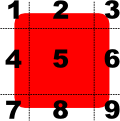
\includegraphics[width=0.7\textwidth]{imgCut}
\caption{{\label{fig:cut}}Diagram ilustrující rozřezání obrázku pomocí elementu \textit{ScaledImage}.}
\end{center}
\end{figure*}

%Každý element, který překryje původní vykreslovací funkci 


\subsection{Zpracování vstupu}
Knihovna přijímá vstup ve formě událostí, které jsou vkládány do fronty pro zpracování. Fronta pro zpracování je realizována pomocí vláknových zámků tak, že pro případ použití ve vícevláknové aplikaci nehrozí, že dojde k problémům, způsobených tím, že více vláken přistupuje k této frontě najednou.
Na počátku fáze \textit{Update} se zavolá funkce \textit{ProcessEvent}s, která má za úkol zpracovat události ve vstupní frontě. Během zpracování jednotlivých událostí se každá událost vybere z fronty, a následně se pošle kořenovému elementu ke zpracování. \\
Události jsou realizovány strukturou \textit{CQMLEvent}, která obsahuje identifikátor druhu události, a konstrukt union, v němž se nachází proměnné typu \textit{CQMLMouseEvent} a \textit{CQMLKeyboardEvent}. To která z těchto dvou proměnných se využije je určeno typem události. Struktura \textit{CQMLMouseEvent} obsahuje data vstupní události vygenerované pomocí myši, konkrétně identifikátor události, hodnotu případného použitého tlačítka, souřadnice myši a případně souřadnice pohybu myši. \textit{CQMLKeyboardEvent} obsahuje identifikátor události vygenerované klávesnicí a hodnotu stisknuté klávesy. Následující seznam vypisuje všechny podporované vstupní události.
\begin{description}
\item[MousePressed] - stisknutí tlačítka myši
\item[MouseReleased] - puštění tlačítka myši
\item[MouseMoved] - pohyb tlačítka myši
\item[MouseScrolled] - pohyb tlačítka myši
\item[KeyPressed] - stisknutí klávesy
\item[KeyReleased] - puštění klávesy
\end{description}
Události se zpracovávají totožným způsobem, element, kterému je předána, ji nejpve předá svým potomkům ke zpracování a následně se ji pokusí zpracovat sám. Samotné zpracování události však závisí na druhu elementu, neboť ty mohou metody pro zpracování překrývat. \\
Události generované klávesnicí se zpracovájí tak, že v případě, že je pro danou událost přiřazena elementu nějaká funkce pro její zpracování (ukazatel na ni není nulový), pak se prostřednictvím ukazatele zavolá.\\
Události generované myší jsou zpracovávány pouze v elementech typu \textit{MouseArea}. U události pro stisk tlačítka myši se pomocí souřadnic a rozměrů elementu a souřadnic myši se ověří zda je ukazatel myši uvnitř daného elementu, pokud ano, vloží se element do pole elementů \textit{pressedElement}. Pokud je elementu přiřazena funkce pro obsluhu této události, pak se zavolá. V případě události pro puštění tlačítka myši se pro všechny elementy v poli \textit{pressedElement} zavolá funkce pro obsluhu této události (byla-li přiřazena), zároveň se u daných elementů zkontroluje, zda se v nich nachází ukazatel myši, pokud tomu tak je, zavolá se funkce pro obsluhu události kliknutí.\\
U události pro pohyb myší se zavolá funkce pro obsluhu, pokud však myš pohybem právě najela na nebo vyjela z oblasti elementu, zavolá se i funkce pro obsluhu jedné z těchto událostí. Při otočením tlačítka myši se u dané události zkontroluje zda se stala uvnitř elementu, je-li tomu tak zavolá se funkce pro jeho obsluhu.\\
Událostí, které lze přiřadit v rámci \textit{CQML} je tak, více než těch, které lze knihovně předat. Následuje seznam vstupních událostí, které lze obsloužit v rámci jazyka \textit{CQML}.
\begin{description}
\item[MousePressed] - stisknutí tlačítka myši (\textit{MouseArea})
\item[MouseReleased] - puštění tlačítka myši (\textit{MouseArea})
\item[MouseClicked] - kliknutí tlačítkem myši (\textit{MouseArea})
\item[MouseMoved] - pohyb tlačítka myši (\textit{MouseArea})
\item[MouseEntered] - pohyb tlačítka myši dovnitř elementu (\textit{MouseArea})
\item[MouseExited] - pohyb tlačítka myši vně elementu (\textit{MouseArea})
\item[MouseScrolled] - pohyb tlačítka myši (\textit{MouseArea})
\item[KeyPressed] - stisknutí klávesy (všechny elementy)
\item[KeyReleased] - puštění klávesy (všechny elementy)
\end{description}



\subsection{Správa externích zdrojů}
Ve fázi Update jednotlivých elementů, se mohli změnit adresy nebo parametry některých elementů používajících externí zdroje, tudíž může být nutné některé zdroje načíst znovu. Proto se u všech elementů, u kterých k tomuto mohlo dojít, uloží do fronty požadavek pro načtení daného externího zdroje. Koknrétně \textit{CQML} elementy Text a Image (stejně tak i elementy z nich odvozené), v rámci metody DefaultUpdate, předávají tyto požadavky pomocí funkcí TryLoadFont a TryLoadImage. Knihovna momentálně podporuje pouze dva druhy externích zdrojů a tím jsou písmo a obrázky. V případě obrázku je takový požadavek definován řetězcem, kterým je cesta k souboru obrázku. V případě písma se jedná o název písma a jeho velikost. \\
%	Deteaily
Na konci fáze \textit{Update} se zpracují všechny požadavky ve frontě. Načtená data jsou v rámci kódu knihovny uchovávána v mapě, která data každého záznamu uchovává ve formě obecného ukazatele typu \textit{void*} ukazující na data načtená data externího zdroje. Jako klíč pro záznam se používá textový řetězec, který je odvozen z požadavku pro načtení. Pro obrázkek je jím opět cesta k souboru a pro písmo je jím jméno písma, za které je do řetězce přidána jeho velikost. V případě, že již byl načten totožný požadavek v minulosti, pak se nebude načítat znovu. To je rozpoznáno tak, že se v mapě již nachází záznam pod daným klíčem. V opačném případě, se prostřednictvím objektu pro obsluhu externích zdrojů, jenž byl ve fázi inicializace knihovně předán, zavolá funkce pro načtení daného externího zdroje, přičemž data následně jsou pod příslušným klíčem uložena do mapy.\\
Kdykoli pak knihovna potřebuje předat uživatelské aplikaci data načtená z externího zdroje, učiní tak předáním \textit{void*} ukazatele uloženého v mapě.\\
Objekt pro obsluhu externí zdrojů, který je knihovně předán v inicializační fázi musí dědit z abstraktní třídy \textit{ResourceManagerIFace} a implementovat její metody. Abstraktní třída \textit{ResourceManagerIFace} vlastní metodu pro načtení písma \textit{LoadFont} a metodu \textit{LoadImage} pro načtení dat obrázku.
%obr?

\subsection{Datový typ \textit{Variant} a \textit{VariantRef}}
Variant je datový typ umožňující manipulaci s hodnotou libovolného datového typu. Účelem typu VarianRef je umožnit obdobnou manipulaci i s referencí na hodnotu libovolného typu.\\

Součástí typu \textit{Variant} je identifikátor typu hodnoty, jaká je uvnitř dané instance uchovávána. Samotnou hodnotu uchovává pomocí konstruktu union, jež obsahuje jeden atribut pro každý datový typ, který je možné v typu \textit{Variant} uchovávat. Jelikož v rámci konstruktu union, nelze uchovávat datové typy s netriviálním konstruktorem, jsou takové typy uchovávány pomocí ukazatele, přičemž jejich hodnota je do typu \textit{Variant} uložena zkopírováním na naalokované místo na haldě a uložením ukazatele na dané místo v paměti pomocí metody \textit{Copy}. Mezi takové typy patří standardní \textit{C++} řetězec a také libovolný datový typ \textit{CQML}. Jelikož všechny \textit{CQML} datové typy dědí ze třídy \textit{CQMLObject}, je ukazatel na takové typy typu ukazatele na obecný \textit{CQMLObject}.\\
Typ \textit{Variant} obsahuje metodu As, která je realizována pomocí čtyř šablon. Tato metoda vrací hodnotu stejného typu, jako je typ, který byl předán jako parametr šablony. Správná šablona je vybrána během kompilace podle jejího parametru. První šablona platí pro číselné typy, metoda As pak v případě, že daná instance typu \textit{Variant} uchovává číselná data vrátí číselnou hodnotu a v opačném případě vyhodí výjimku. Druhá šablona provádí totéž pro řetězcová data. Třetí šablona činí totéž pro ukazatele na objekt typu \textit{CQMLObject}. Čtvrtá šablona je pro ostatní datové typy a ta vždy vyhodí výjimku.
Typ \textit{Variant} implementuje několik přetížených konstrukturů, každý z nich inicializuje identifikátor typu hodnoty a následně uloží hodnotu, která mu byla v parametrech předána.\\
Typ \textit{Variant} přetěžuje základní aritmetické operátory, všechny operátory nejprve zjistí zda typ levého operandu podporuje danou operaci a následně se pokusí pravý operand přetypovat pomocí metody As na stejný typ, jakým je levý operand. V případě úspěchu se daná operace provede. Pro většinu nečíselných typů nejsou podporovány aritmetické operace. Výjimkou je operace sčítání, která je implementována i pro řetězce. Pokud některý typ nepodporuje určitou aritmetickou operaci, pak při zavolání daného operátoru dojde k vyhození výjimky.\\
Typ \textit{Variant} implementuje metodu \textit{Get}, která v případě, že je v něm uchovávána hodnota typu \textit{CQMLObject}, zavolá tutéž metodu na daný \textit{CQMLObject} a vrátí vrácenou hodnotu. Pro hodnoty ostatních typů vyhodí výjimku.

Součástí datového typu \textit{VariantRef} je identifikátor typu hodnoty, na kterou ukazuje daná instance. Samotný ukazatel se uchovává pomocí konstruktu union, jež obsahuje jeden atribut pro každý typ ukazatele. Narozdíl od typu \textit{Variant} je zde pro \textit{CQML} typy rozlišováno zda se jedná o datové či hodnotové typy. Také je zde uchováván ukazatel na ukazatel funkce pro přepočítání atributu.\\
VariantRef také implementuje metodu \textit{As}, avšak narozdíl od typu \textit{Variant}, je realizována pomocí jedné šablony, která přijímá návratový typ jako parametr. Daná metoda pouze přetypuje daný objekt na typ \textit{Variant} a zavolá jeho metodu \textit{As}.\\
VariantRef přetěžuje podobně jako typ \textit{Variant} operátory. V případě operátorů pro přiřazení, však dojde ke změně hodnoty, na kterou typ \textit{Variant} ukazoval. Jelikož se typ \textit{VariantRef}t používá pro přímý přístup k atributu nějakého elementu, dojde při změně hodnoty k vynulování ukazatele na funkci, jež slouží pro přepočítávání hodnoty daného atributu. V případě ostatních operátorů se levý operand přetypuje na typ \textit{Variant} a provede se operace, která byla implementována v rámci přetíženého operátoru ve třídě \textit{Variant}. Metoda \textit{Get} je zde realizována totožným způsobem jako u typu \textit{Variant}.

Typy \textit{Variant} a \textit{VariantRef} podporují uložení následujících datových typů:
\begin{itemize}
\item číselné typy - \textit{int}, \textit{long}, \textit{long long} (\textit{signed} i \textit{unsigned}), \textit{float}, \textit{double}, \textit{long double}
\item řetězec - \textit{string}, \textit{char*}
\item libovolný datový \textit{CQML} typ - \textit{CQMLObject*}
\item obecný ukazatel - \textit{void*}
\end{itemize}

\subsection{Datové typy \textit{CQML}}
Všechny datové typy přístupné v rámci jazyka \textit{CQML}, které nejsou primitivními typy, dědí z datového typu \textit{CQMLObject}. Třída \textit{CQMLObject} obsahuje člen \textit{classID}, který v sobě uchovává identifikátor třídy. Dále obsahuje virtuální metodu \textit{Copy}, pro zkopírování aktuální instance, a také virtuální metodu \textit{Get}, která slouží pro přístup k libovolnému atributu. Metoda \textit{Get} jako parametr přijímá název atributu, který by měl být členem dané struktury. Tato metoda podle hodnoty haše vypočteného pomocí hašovací funkce z názvu vybere příslušný atribut, přičemž hašovací funkce je vybrána podle identifikátoru \textit{classID}. Tato metoda vrací hodnotu typu \textit{VariantRef}, do kterého se uloží adresa daného atributu a také adresa ukazatele na funkci pro jeho zpracování.\\

\section{Uživatelská aplikace}
Pro účely demonstrace funčnosti knihovny jím generovaného \textit{GUI} bylo nutné vytvořit testovací aplikaci, která by umožnila použití \textit{CQML} knihovny.
Pro účely vstupu a vykreslování je použita knihovna \textit{SDL2}. Pro použití knihovny je nutno implementovat třídy, jež implementují rozhraní pro vykreslování a správu externích zdrojů. Pro účely vykreslování je vytvořena třída \textit{SDL\_Drawer}, která dědí z abstraktní třídy \textit{DrawIFace}. Pro správu externích zdrojů slouží třída \textit{SDL\_Manager} dědící z abstraktní třídy \textit{ResourceManagerIFace}.\\
Na počátku programu se inicializuje knihovna \textit{SDL}. Následně se spustí inicializace \textit{CQML} knihovny metodou \textit{\_CQML\_Init}. Poté se vytvoří instance třídy \textit{SDL\_Drawer} a \textit{SDL\_Manager}, jež se předají runtime \textit{CQML} knihovně. A na závěr inicializace se zavoláním metody \textit{\_CQML\_Start} ukončí inicializace. Pomocí metody GetCQMLWindow knihovny \textit{CQML} získají rozměry kořenového elementu v GUI hierarchii.
Následně se vytvoří okno a spustí se hlavní programová smyčka. Hlavní programová smyčka se skládá ze tří fází – zpracování vstupu, update, vykreslování.
Knihovna \textit{SDL} zpracovává vstup jako frontu vstupních událostí. Proto se ve fázi pro zpracování vstupu vyjmou z fronty všechny vstupní události a postupně se přeformují do formátu přijímaného knihovnou \textit{CQML} a pomocí metody \textit{PushEvent} se knihovně \textit{CQML} odešlou. Ve fázi update se spustí funkce \textit{\_CQML\_Update} čímž se aktualizují hodnoty elementů uvnitř \textit{GUI} hierarchie. Ve fázi vykreslení se na počátku vyčistí obrazovka a následně se vykreslí \textit{GUI} hierarchie pomocí funkce \textit{\_CQML\_Draw}. Hlavní programová smyčka běží, dokud uživatel nestiskne křížek pro zavření okna, který vyvolá vstupní událost \textit{SDL\_QUIT}, která smyčku ukončí, což vede k uvolnění zdrojů a ukončení programu.\\
\textit{SDL\_Manager} implementuje metodu pro načtení písma LoadFont, která pomocí funkce \textit{TTF\_OpenFont} knihovny \textit{SDL\_TTF} načte požadovaný font a vrátí na něj ukazatel. Také implementuje metodu pro načtení obrázků pomocí knihovny \textit{SDL\_image}, která pomocí funkce \textit{IMG\_Load} načte data obrázku. Načtená data obrázku jsou uložena spolu s rozměry obrázku do struktury \textit{ImageData}, která je následně metodou vrácena. 
\textit{SDL\_Drawer} implementuje vykreslovací metody abstraktní třídy \textit{DrawIface}. Tyto metody jsou realizovány pomocí vykreslovacích funkcí poskytovaných knihovnou \textit{SDL}.

\chapter{\label{CH:conc}Výsledky}
\section{\label{SEC:Conclusion}Srovnání tvorby jednoduchého rozhraní pomocí \textit{CQML} a \textit{QML}}
Srovnání funkčnosti je ilustrováno na jednoduché \textit{GUI} aplikaci. Aplikace má několik částí. Obsahuje hlavní nabídku s několika tlačítky, kalkulačku a jednoduchou hru. V nabídce uživatel může kliknutím na příslušné tlačítko vybrat část aplikace, která se následně spustí.\\
Jednotlivé části aplikace jsou realizovány pomocí samostatných komponent. Základní funkčnost \textit{QML} ani \textit{CQML} nepodporuje tvorbu více oken, tudíž není možné rozdělit komponenty do samostatných oken. Z tohoto důvodu je přepínání mezi částmi aplikace řešeno jejich skrytím a odkrytím prostřednictvím nastavení hodnoty parametru pro viditelnost.
\subsection{Hlavní nabídka}
Jednoduchá nabídka, jenž obsahuje tři tlačítka. První tlačítko zobrazí rozhraní kalkulačky, druhé zobrazí rozhraní hry a třetí ukončí program.
\subsubsection{QML Realizace}
Tlačítko v nabídce je realizováno jako samostatná komponenta \textit{TextButton}.  Kořenovým elementem v této komponentě je \textit{MouseArea}. Tlačítku jsou přiřazeny metody pro zpracování událostí, pro najetí ukazatelem myši na plochu vymezenou tlačítkem ukazatele myši a také na její opuštění, dále jsou přiřazeny metody pro stisknutí a puštění tlačítka myši na daném elementu. Tyto metodu slouží pro přepínání obrázku tlačítka. Kořenový element má dva potomky - jeden typu \textit{Text} a druhý typu \textit{Image}. Element \textit{Text} zde slouží pro zobrazení textu na tlačítku a image slouží k zobrazení obrázku tlačítka. Cesty k obrázkům jsou uloženy do přidaných řetězcových atributů a jsou celkem tři – základní obrázek, obrázek po najetí myší na tlačítko a obrázek po jeho stisknutí. \\
Při manipulaci s komponentou zvenčí je možné přistupovat pouze k atributům, které vlastní kořenový prvek komponenty. Aby tak bylo možné vytvářet pomocí této komponenty tlačítka s různým popiskem, je do kořenového prvku pomocí příkazu alias přidán odkaz na atribut text elementu \textit{Text} pro zobrazení textu.
Nabídka se nachází na vrcholu celé \textit{GUI} hierarchie, tudíž jejím kořenovým elementem je element typu \textit{Window}. Ten obsahuje dvě hlavní komponenty (kalkulačku a hru), jejichž viditelnost je vypnuta, dále obsahuje tři tlačítka vytvořená z komponenty \textit{TextButton}. Každé tlačítko má přiřazeno funkci pro obsluhu události kliknutí. V případě prvních dvou tlačítek tato funkce vypne viditelnost všech tlačítek a zapne viditelnost jedné z hlavních komponent. Třetí tlačítko v případě kliknutí vyšle signál k ukončení aplikace. Na obrázku \ref{fig:outMenuQML} je ukázáno vygenerované \textit{GUI}.
\begin{figure*}[!ht]
\begin{center}
  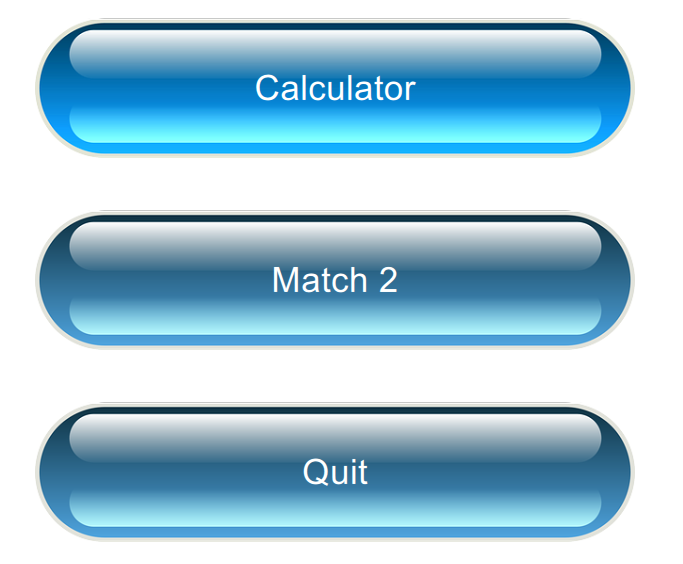
\includegraphics[width=0.7\textwidth]{qmlMenu}
\caption{{\label{fig:outMenuQML}}Obrázek jednoduché nabídky realizované v jazyce \textit{QML}.}
\end{center}
\end{figure*}

\subsubsection{\label{SEC:CQMLMenu}CQML Realizace}
Realizace nabídky v rámci \textit{CQML} je téměř totožná s realizací pomocí \textit{QML}, zanedbají-li se rozdíly v syntaxi obou jazyků.
Stejně jako je tomu u \textit{QML}, \textit{CQML} umožňuje z vnějšku komponenty přímo manipulovat pouze s atributy kořenového prvku dané komponenty. \textit{CQML} na rozdíl od \textit{QML} ale neumožňuje vytvoření odkazu na atribut elementu. Tudíž k němu není možné přímo přistupovat.  V tomto případě je to však vyřešeno tak, že kořenovému prvku je přiřazen identifikátor \textit{thisButton} a zároveň je do něj přidán nový atribut jménem \textit{buttonLabel} typu řetězec. V příkazu pro určení hodnoty atributu text elementu \textit{Text} je následně výrazem \textit{thisButton.buttonLabel} určeno, že se má použít hodnota \textit{buttonLabel} kořenového elementu. Tímto způsobem tak lze nepřímo měnit hodnotu zobrazovaného textu z vnějšku komponenty. Na obrázku \ref{fig:outMenuCQML} se nachází rozhranní vygenerované z \textit{CQML} kódu.
\begin{figure*}[!ht]
\begin{center}
  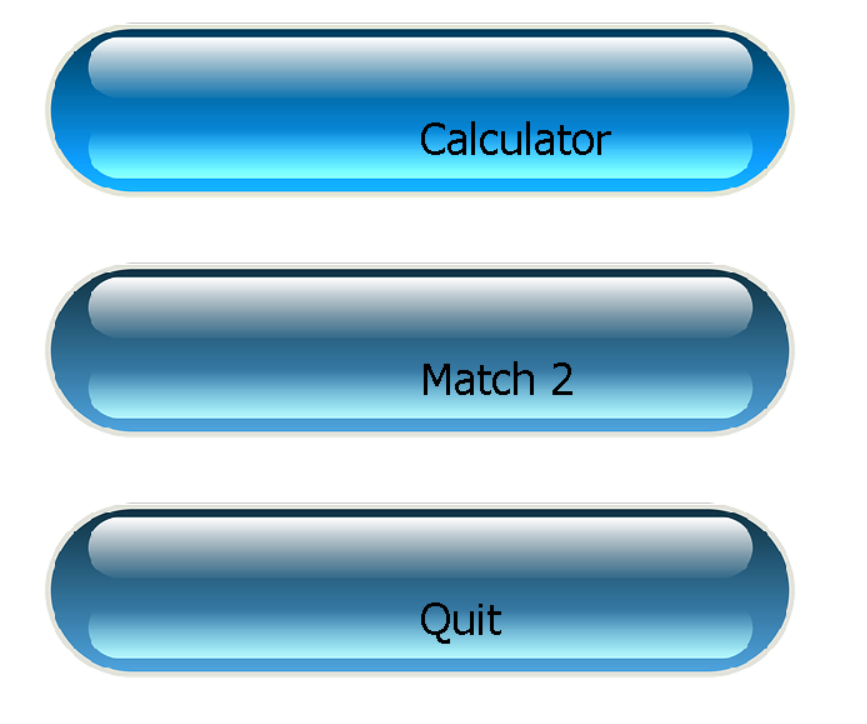
\includegraphics[width=0.7\textwidth]{cqmlMenu}
\caption{{\label{fig:outMenuCQML}}Obrázek jednoduché nabídky realizované v jazyce \textit{CQML}.}
\end{center}
\end{figure*}

\subsection{Kalkulačka}
Cílem této části je vytvořit jednoduchou kalkulačku. Kalkulačka umožní uživateli zadávat čísla a provádět základní aritmetické operace Kalkulačka obsahuje zobrazovací řádek pro zobrazení zadávaného čísla, který ale také slouží pro zobrazení výsledku operace. Dále aplikace obsahuje deset tlačítek pro zadání jednotlivých číslic, tlačítko pro vynulování, tlačítko pro spuštění zadávání desetinné části a pět tlačítek reprezentující aritmetické operátory plus, mínus, děleno, krát a rovná se. V této části bude využita externí funkčnost a to tak, že každé tlačítko bude volat příslušnou funkci z externího souboru.
\subsubsection{QML Realizace}
Řádek pro výstup je realizován pomocí elementu \textit{BorderImage}, jež zobrazí jako obrázek okraje řádku, na který se vypisuje výstup kalkulačky. Tento element v sobě obsahuje jednoho potomka typu Text označeného identifikátorem \textit{thisText}, který slouží k zobrazení textového výstupu kalkulačky.
Všechna tlačítka jsou realizována pomocí komponenty \textit{CalculatorButton}.  Komponenta \textit{CalculatorButton} se skládá z pouze jednoho elementu, kterým je komponenta \textit{TextButton}, které je nastavena šířka a výška a odlišné cesty ke zdrojovým obrázkům, než má nastavené výchozí \textit{TextButton}.\\ Každé tlačítko má přiřazenou funkci pro obsluhu událostí, která volá funkce externí logiky importované ze souboru "CalcLogic.js". Každá externě volaná funkce v tomto případě představuje operaci kalkulačky, kterou má provést po stisknutí tlačítka, přičemž vrací hodnotu, která se má zobrazit na výstupním řádku kalkulačky, tato hodnota se přiřadí elementu označenému \textit{thisText}, který jí zobrazí. Obrázek \ref{fig:outCalcQML} ukazuje výsledné rozhraní.
\begin{figure*}[!ht]
\begin{center}
  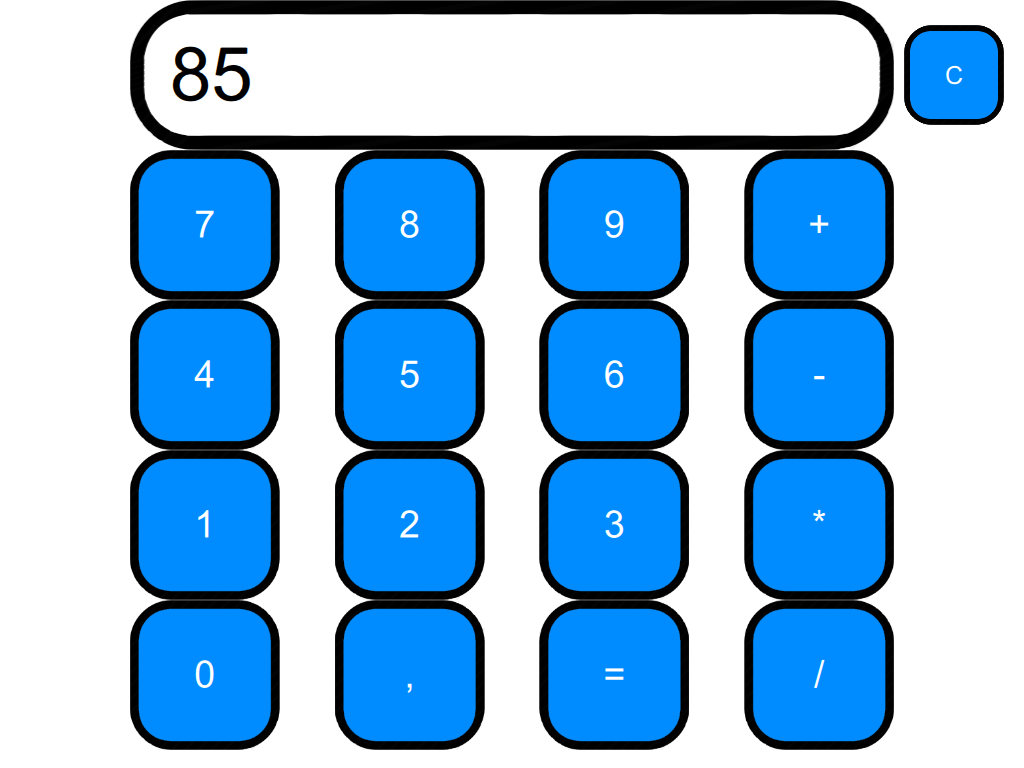
\includegraphics[width=0.7\textwidth]{qmlCalc}
\caption{{\label{fig:outCalcQML}}Obrázek kalkulačky realizované pomocí deklarace v jazyce \textit{QML}.}
\end{center}
\end{figure*}

\subsubsection{CQML Realizace}
CQML realizace je v mnoha směrech podobná, avšak s několika rozdíly. Veškerá logika kalkulačky je implementována v rámci uživatelské aplikace v jazyce \textit{C++}. Pomocí příkazu include je do \textit{CQML} zahrnut hlavičkový soubor „calc\_logic.h“. V tomto souboru je definovaná struktura \textit{CalculatorLogic}, která slouží pro obsluhu aplikační logiky kalkulačky a je zde také deklarovaná proměnná typu této struktury s názvem \textit{CalcLogic}. V rámci funkcí uvnitř \textit{CQML} kódu pak lze k dané proměnné přistupovat a volat její metody. Jednotlivá tlačítka mají přiřazena funkci pro obsluhu události kliknutí, z nichž každá volá příslušnou metodu struktury \textit{CalculatorLogic}. Obrázek \ref{fig:outCalcCQML} ukazuje výsledné rozhraní realizované v \textit{CQML}.
\begin{figure*}[!ht]
\begin{center}
  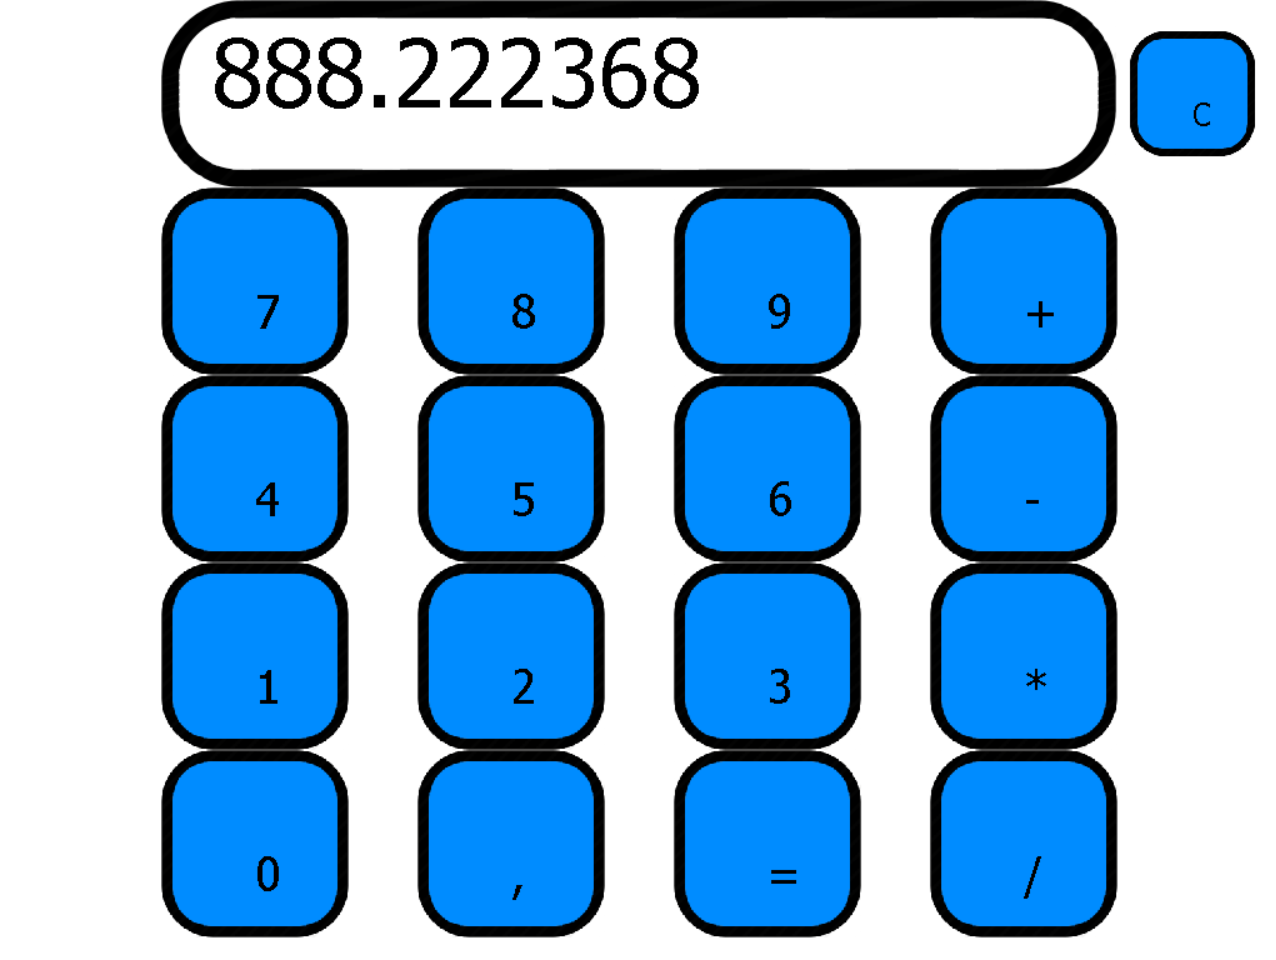
\includegraphics[width=0.7\textwidth]{cqmlCalc}
\caption{{\label{fig:outCalcCQML}}Obrázek kalkulačky realizované pomocí deklarace v jazyce \textit{CQML}.}
\end{center}
\end{figure*}



\subsection{Jednoduchá hra}
Pro ilustraci možností používání dynamických referencí na atributy poslouží hra s velmi jednoduchými pravidly. Na herní ploše je rozmístěno několik různě barevných hracích kamenů, pro účely aplikace budou ve formě tlačítek. Úkolem hráče je označit dvě stejně barevná tlačítka tak, že na ně klikne pomocí myši. Pokud hráč označí tlačítka s různou barvou, pak vybírá znovu. Při správném označení dvou tlačítek stejné barvy, obě tlačítka jsou odstraněna a hráči jsou přičteny body k jeho celkovému skóre. Hráčovo skóre se zobrazuje v zobrazovacím řádku.
\subsubsection{QML Realizace}
Jednotlivá tlačítka představující hrací kameny jsou realizována pomocí komponent \textit{GameCircle}, který je odvozen z komponenty \textit{NormalButton}, podobně jako \textit{CalculatorButton} je odvozen z \textit{TextButton}. \textit{NormalButton} je komponenta s totožnou funkčností jako \textit{TextButton}, jen neobsahuje funkčnost pro zobrazení popisku tlačítka.
Hrací plocha je reprezentována elementem typu \textit{Rectangle}, který je rozšířen o několik atributů. Hrací plocha obsahuje element \textit{Text} pro zobrazení vítězné zprávy, šestnáct elementů typu \textit{GameCircle}, které jsou umístěny v elementu typu \textit{Grid}, který je všechny rozmístí do zadaného počtu sloupců a řádků. Element představující hrací plochu je rozšířen o několik celočíselných atributů pro uchování hodnoty hráčova skóre, aktuálního stavu a hodnoty předchozího vybraného hracího kamene, další dva přidané atributy slouží k uchování reference na předchozí hrací kámen a na element pro zobrazení vítězné zprávy.\\
Kořenovým elementem komponenty \textit{GameCircle} je element typu \textit{NormalButton}, který je rozšířen o dva atributy – value a matcher. Atribut value udává hodnotu herního kamene a matcher uchovává referenci na element představující hrací plochu. Obrázky, které určují vzhled tlačítka, jsou vybírány podle hodnoty herního kamene. Dále je kořenovému elementu této komponenty přiřazena funkce pro obsluhu události kliknutí. Daná funkce prostřednictvím reference matcher přistupuje k atributům hrací plochy, pomocí nichž zjistí, zda je vybrán nějaký hrací kámen. Není-li tomu tak, je následně v hrací ploše uložena reference na hrací kámen, na nějž bylo kliknuto. Byl-li již nějaký hrací kámen vybrán, je zkontrolováno, zda má stejnou hodnotu s kamenem, na který bylo právě kliknuto. Pokud mají stejnou hodnotu, je přičtena hodnota kamene k hráčovu skóre a oba hrací kameny jsou smazány. V opačném případě je smazána reference na předchozí vybraný kámen a hráč musí vybrat oba kameny znovu. Jsou-li všechny kameny smazány, což se pozná kontrolou maximální hodnoty skóre, je prostřednictvím reference matcher na hrací plochu přistoupeno k elementu pro zobrazení vítězné zprávy a zapne se její viditelnost. Obrázek \ref{fig:outGameQML} ilustruje vzhlede rozhranní po odebrání několika herních kamenů.
\begin{figure*}[!ht]
\begin{center}
  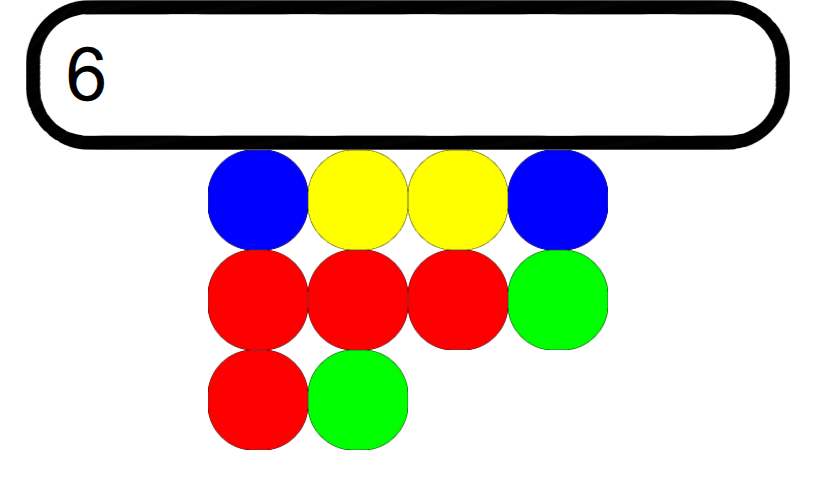
\includegraphics[width=0.7\textwidth]{qmlGame}
\caption{{\label{fig:outGameQML}}Obrázek jednoduché hry realizované pomocí deklarace v jazyce \textit{QML}.}
\end{center}
\end{figure*}

\subsubsection{CQML Realizace}
Na rozdíl od \textit{QML} aktuální verze \textit{CQML} neumožňuje užívání elementů pro automatické rozvržení, jakými jsou například \textit{Grid}, \textit{Row}, \textit{Column}. Z tohoto důvodu je nutné v \textit{CQML} souboru ručně zapsat souřadnice jednotlivých hracích kamenů resp. tlačítek.
CQML neumožňuje dynamickou tvorbu a mazání elementů, proto nejsou při správném výběru hrací kameny smazány a pouze se skryjí.
Na obrázku \ref{fig:outGameCQML} je vidět vygenerované rozhranní, po odebrání několika herních kamenů, oproti výsledku zobrazeném v \textit{QML} realizaci se po odebrání kamene ostatní kameny neseřadí (přávě toto v \textit{QML} obstarává element \textit{Grid}).
\begin{figure*}[!ht]
\begin{center}
  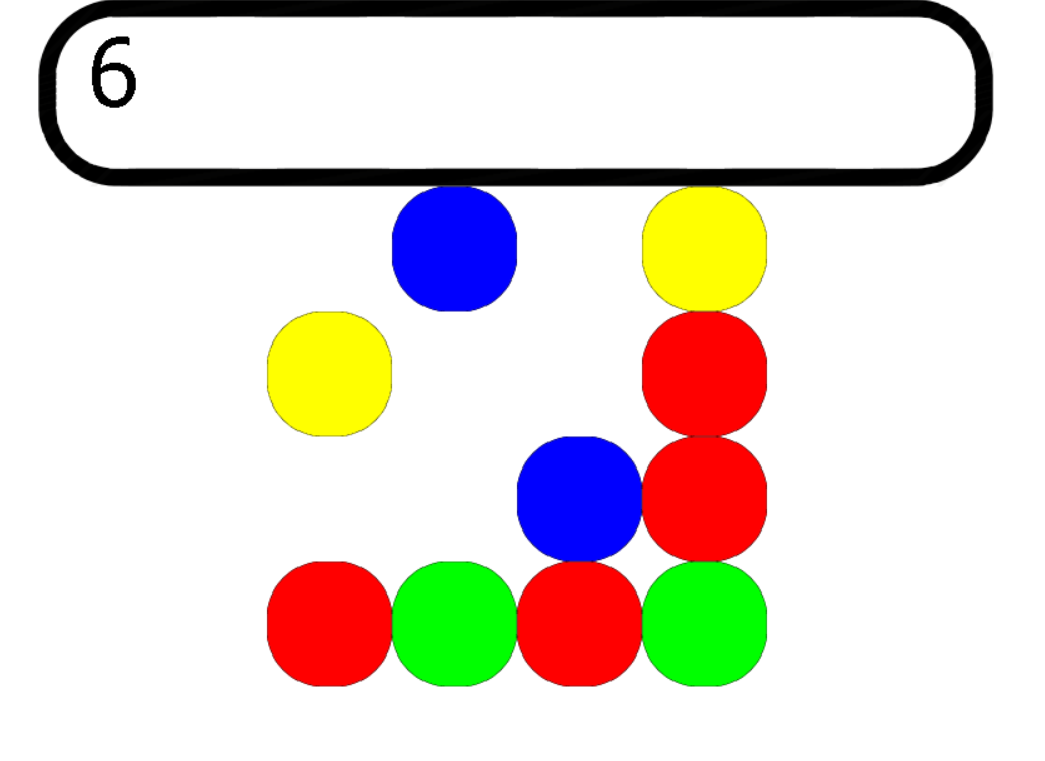
\includegraphics[width=0.7\textwidth]{cqmlGame}
\caption{{\label{fig:outGameCQML}}Obrázek jednoduché hry realizované pomocí deklarace v jazyce \textit{CQML}.}
\end{center}
\end{figure*}

\section{Porovnání \textit{QML} a \textit{CQML}}
Základní syntaxe a funkčnost jazyků \textit{CQML} a \textit{QML} je velmi podobná. Hlavním rozdílem je, že zatímco jazyk \textit{QML} je interpretován (ať už ve své textové podobě či po překladu do byte-kódu) v rámci uživatelské aplikace, tak jazyk \textit{CQML} slouží pro vygenerování zdrojových kódů v jazyce \textit{C++}, které jsou přímo do uživatelské aplikace vloženy a jsou překládány spolu s ní.\\
Knihovna, která za běhu obsluhuje hierarchii vygenerovanou z jazyka \textit{CQML} umožňuje uživateli použít vlastní funkce pro vykreslování a správu zdrojů (obrázků a písem), ovšem na rozdíl od knihovny \textit{QML} neposkytuje vlastní funkčnost pro tento účel.
Oba jazyky mimo jiné umožňují dynamicky provázat atributy elementů, přidávání nových atributů, přiřazování funkcí pro obsluhu vstupních událostí a tvorbu nových komponent. Oba jazyky podporují zapouzdření funkčnosti \textit{GUI} do samostatných souborů (komponent), které mohou být následně využívány, jako samostatné elementy v rámci jiné \textit{GUI} hierarchie.\\
Nevýhodou \textit{CQML} oproti \textit{QML} je výrazně menší počet podporovaných grafických elementů. \textit{CQML} momentálně poskytuje jen několik základních elementů, zatímco \textit{CQML} poskytuje několik stovek elementů s odlišnou funkčností.\\
Za výhodu knihovny \textit{CQML} lze považovat, že se nachází pod volnější open-source licencí než prostředí \textit{Qt}, jehož součástí je knihovna \textit{QML}. Zatímco \textit{CQML} je dostupné pod licencí \textit{BSD}, \textit{Qt} spadá pod licenci \textit{LGPL}. \textit{QML} tak nelze například použít v rámci komerčních aplikací, které nejsou open-source.
Následuje popis hlavních rozdílů týkajících se možností realizace funkčnosti GUI.
\subsection{Tvorba více oken}
Oba jazyky nepodporují tvorbu více oken uvnitř GUI Hierarchie, jazyk \textit{QML} však umožňuje v rámci uživatelské aplikace v jazyce \textit{C++} spustit několik samostatných instancí GUI, mezi kterými je možno přepínat, to pro knihovnu \textit{CQML} není možné.
\subsection{Reference na atributy}
Jazyk \textit{QML} umožňuje v rámci elementu pomocí klíčového slova \textit{alias} vytvářet reference na atributy jiných elementů. V jazyce \textit{CQML} toto není možné, avšak tento problém se dá v některých případech obejít, jak je ilustrováno v \ref{SEC:CQMLMenu}.
\subsection{Dynamická změna hierarchie elementů}
QML jazyk umožňuje dynamicky měnit hierarchii elementů pomocí mazání a přidávání elementů či komponent za běhu programu pomocí vyhrazených funkcí a metod. \textit{CQML} jazyk aktuálně takovou možnost nemá. \textit{QML} knihovna dále umožňuje za běhu načítat nové soubory jazyka \textit{QML} a používat uvnitř definované GUI. Knihovna pro jazyk \textit{CQML} toto už z principu neumožňuje, jelikož se jazyk překládá do nativního kódu \textit{C++} a tudíž musí být všechny používané \textit{CQML} soubory zpracovány a přeloženy ještě před spuštěním uživatelské aplikace.
\subsection{Rozšiřitelnost}
Jazyk \textit{QML} může být rozšířen o nové elementy pomocí jejich implementace v uživatelské \textit{C++} aplikaci. Nový element je představován třídou, která dědí z třídy \textit{QObject}, a její vlastnosti, které mají být přístupné z jazyka \textit{QML}, musí být deklarovány pomocí speciálních maker. 
Jazyk \textit{CQML} může být také rozšířen o nové elementy. Pro vytvoření nového elementu je potřeba definovat název, atributy a metody daného elementu pomocí speciálních maker v rámci hlavičkového souboru, který je pro to určen (viz. sekce \ref{SEC:header}). Po definici nových elementů pomocí těchto maker, musí být spuštěn preprocesor vestavěných datových typů, který vygeneruje kód, který se zahrne do runtime knihovny. V rámci knihovny je nutno implementovat funkčnost nových elementů a následně knihovnu zkompilovat. Teprve poté je možno nový vestavěný element použít.


\section{Závěr}
Během této práce byl pečlivě prozkoumán jazyk \textit{QML} pro deklarativní definici \textit{GUI}. Na jeho základě byl navržen jazyk \textit{CQML} s podobnou syntaxí a byla vytvořena jeho gramatika. Jazyk \textit{CQML} může být rozšířen o další grafické elementy, které mohou být definovány v samostatných \textit{CQML} souborech, takové elementy musí vycházet z již existujících. V základu však \textit{CQML} neposkytuje takové množství grafických elementů jako jazyk \textit{QML}.\\
Podařilo se vytvořit překladač, který vygeneruje zdrojový kód pro \textit{GUI} definované pomocí jazyka \textit{CQML}. Vygenerovaný kód je v jazyce \textit{C++} a lze jej přímo zahrnout do kódu uživatelské aplikace, která jej zobrazí.\\
Pro správu \textit{GUI} hierarchie v rámci uživatelské aplikace byla vytvořena runtime knihovna, která tuto funkčnost obstará. Knihovna podporuje vyměnitelné externí rozhraní pro vstup a výstup, který musí být poskytnut uživatelskou aplikací. Komunikace s uživatelskou aplikací je prováděna pomocí rozhraní pro vstup a výstup. 
Rozšíření základní funkčnosti knihovny, které nelze realizovat tvorbou nových komponent v rámci \textit{CQML} souborů, vyžaduje zásah do zdrojových kódů knihovny. Aplikace byla navržena tak, aby byla rozšiřitelnost co nejjednodušší, tudíž se nové typy elementů deklarují v jednom souboru pomocí speciálních maker, který je sdílen mezi všemi částmi \textit{CQML} aplikace s tím, že nová funkčnost přidaných typů elementů musí být implementována pouze v kódu runtime knihovny. Kód pro samotnou integraci nového elementu do jazyka \textit{CQML} je generován automaticky. Je však stále nutné všechny části aplikace znovu přeložit.\\
Pro testovací účely byla naprogramována uživatelská aplikace, která využívá runtime knihovnu \textit{CQML} a implementuje externí rozhraní pro vstup a výstup pomocí knihovny \textit{SDL2}. Dále bylo vytvořeno uživatelské rozhranní v jazyce \textit{CQML} a \textit{QML}, na kterém byla demonstrována funkčnost tvorby \textit{GUI} v jazyce \textit{CQML} a také srovnání definice \textit{GUI} v obou jazycích.\\
Knihovna \textit{CQML} je poskytována jako open-source pod volnou \textit{BSD} licencí. Knihovnu je možné nadále rozvíjet a rozšiřovat její funkčnost, včetně přidávání dalších grafických elementů.





\bibliographystyle{csplainnat}
\begin{thebibliography}{99}
\bibitem{bib:hashPerfect} An optimal algorithm for generating minimal perfect hash functions -- Zbigniew J. Czech, George Havas, Bohdan S. Majewski, 1992; \url{http://cmph.sourceforge.net/papers/chm92.pdf}, stav z 10.\,5.\,2013
\bibitem{bib:wxSmith} WxSmith plugin -- \url{http://wiki.codeblocks.org/index.php?title=WxSmith_plugin}, stav z 10.\,5.\,2013
\bibitem{bib:swingBuilder} Swing GUI Builder -- \url{https://netbeans.org/features/java/swing.html}, stav z 10.\,5.\,2013
\bibitem{bib:ultimate} Ultimate++ Overview -- \url{http://ultimatepp.org/www$uppweb$overview$en-us.html}, stav z 10.\,5.\,2013
\bibitem{bib:UIML} UIML: an appliance-independent XML user interface language -- Marc Abrams, Constantinos Phanouriou, Alan L. Batongbacal, Stephen M. Williams, Jonathan E. Shuster; \url{http://www.ramb.ethz.ch/CDstore/www8/data/2170/pdf/pd1.pdf}, stav z 10.\,5.\,2013
\bibitem{bib:XAML} XAML Overview (WPF) -- \url{https://msdn.microsoft.com/en-us/library/ms752059.aspx}, stav z 10.\,5.\,2013
\bibitem{bib:FXML} Introducing FXML: A Markup Language for JavaFX -- Greg Brown, 2011; \url{http://fxexperience.com/wp-content/uploads/2011/08/Introducing-FXML.pdf}, stav z 10.\,5.\,2013
\bibitem{bib:MXML} Developing applications in MXML -- \url{http://help.adobe.com/en_US/flex/using/WS2db454920e96a9e51e63e3d11c0bf5f39f-7fff.html}, stav z 10.\,5.\,2013
\bibitem{bib:boost} Boost Variant -- Eric Friedman, Itay Maman, 2003 \url{http://www.boost.org/doc/libs/1_54_0/doc/html/variant.html#variant.abstract}, stav z 10.\,5.\,2013
\bibitem{bib:history} A History of the GUI -- Jeremy Reimer, 2005, \url{http://www.cdpa.co.uk/UoP/Found/Downloads/reading6.pdf}, stav z 10.\,5.\,2013
\bibitem{bib:model} Automatic User Interface Generation from Declarative Models -- Egbert Schlungbaum, Thomas Elwert, 1995; \url{http://www.usixml.org/servlet/Repository/schlungbaum-cadui96.pdf?ID=331}, stav z 10.\,5.\,2013
\bibitem{bib:AHI} AUGMENTING HUMAN INTELLECT: A Conceptual Framework -- D. C. Engelbart, 1962; \url{http://www.invisiblerevolution.net/engelbart/full_62_paper_augm_hum_int.html}, stav z 10.\,5.\,2013
\bibitem{bib:PARC} Xerox PARC history -- \url{https://www.parc.com/about/}, stav z 10.\,5.\,2013
\bibitem{bib:aug} A Research Center for Augmenting Human Intellect -- Douglas C. Engelbart, William K. English, 1968; \url{http://www.dougengelbart.org/pubs/augment-3954.html}, stav z 10.\,5.\,2013
\bibitem{bib:model2} A Model-Based Interface Development Environment -- ANGEL R. PUERTA, 1997
\end{thebibliography}


\appendix
\chapter{\label{CH:APA}Příloha A - Gramatika }
Následuje soubor pravidel pro gramatiku ve formátu \textit{YACC} pro jazyk \textit{CQML}. Terminály jsou psané velkým písmem a neterminální symboly malým. Neterminály "compound\_statement", "type\_specifier" a "conditiona\_lexpression" jsou převzaty z gramatiky pro jazyk C, a jejich zpracování bude provedeno podle pravidel gramatiky jazyka C.
\begin{lstlisting}[frame=single,caption=Gramatika jazyka \textit{CQML},label=lst:g]
start_point
	:	element_or_import_list
;

element_or_import_list
	:	import_list element
	|	element
;

import_list
	:	import import_list
	|	import
;

import
	:	IMPORT STRING_LITERAL AS IDENTIFIER
;
element
	:	IDENTIFIER '{' attribute_or_subelement_list '}'
	|	IDENTIFIER '{' '}'
;
attribute_or_subelement_list
	: attribute_or_element ';' attribute_or_subelement_list
	| attribute_or_element ';'
;


attribute_or_element
	: element
	| event_handler
	| attribute
	| property
;


event_handler
	: IDENTIFIER ':' compound_statement
;

property
	: PROPERTY IDENTIFIER attribute
	| PROPERTY type_specifier attribute
	| PROPERTY IDENTIFIER IDENTIFIER
	| PROPERTY type_specifier IDENTIFIER
;


attribute
	:	IDENTIFIER ':' conditional_expression
	|	IDENTIFIER '.' IDENTIFIER ':' conditional_expression
;
\end{lstlisting}

\clearpage
\chapter{\label{CH:APB}Příloha B - Použité technologie }

\subsubsection{Flex}
\textit{Flex} je nástroj pro tvorbu skenerů pro lexikální analýzu. Jeho cílem je rozpoznat lexikální šablony v textovém vstupu a převést je na výstup ve formě posloupnosti symbolů (tokenů), které mohou být zpracovány dále například pomocí parseru.
\subsubsection{Bison}
\textit{Bison} je víceúčelový generátor parserů, který z dané bezkontextové gramatiky vygeneruje deterministický LR parser nebo generalizovaný LR parser ve formě zdrojového kódu k programu v jazyce \textit{C} nebo \textit{C++}.
\subsubsection{SDL2}
\textit{SDL2} je multiplatformní knihovna umožňující přístup ke vstupním a výstupním zařízením systému. Podporuje platfromy \textit{Windows}, \textit{Mac OS X}, \textit{Linux}, \textit{iOS} a \textit{Android}. Je implementován v kódu jazyka \textit{C} a tak jí lze použít i v rámci \textit{C++} aplikací.

\end{document}
